\section{Simple Techniques}
    \subsection{Simple Spirals}
        Spirals can be created by a simple pattern (Fig. \ref{spiral_setup_01}).
        First a identity segment is drawn then, a single segment recurses further.
        We can call the segment that recurses further, \emph{the recursive segment}.
        The type of the spiral depends on the placement of the recursive segment (green in this case).

        \begin{figure}[ht]
            \caption{\label{spiral_setup_01} Setup of a spiral.}
            \centering
            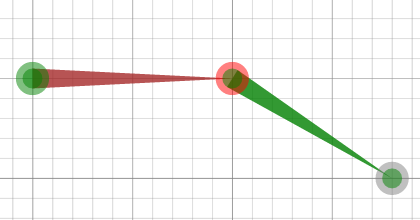
\includegraphics[width=0.4\textwidth]{img/Simple_Techniques/Spirals/spiral_setup_01.png}
        \end{figure}

        \begin{figure}[ht]
            \caption{\label{spiral_simple_01} Simple spirals.}
            \centering
            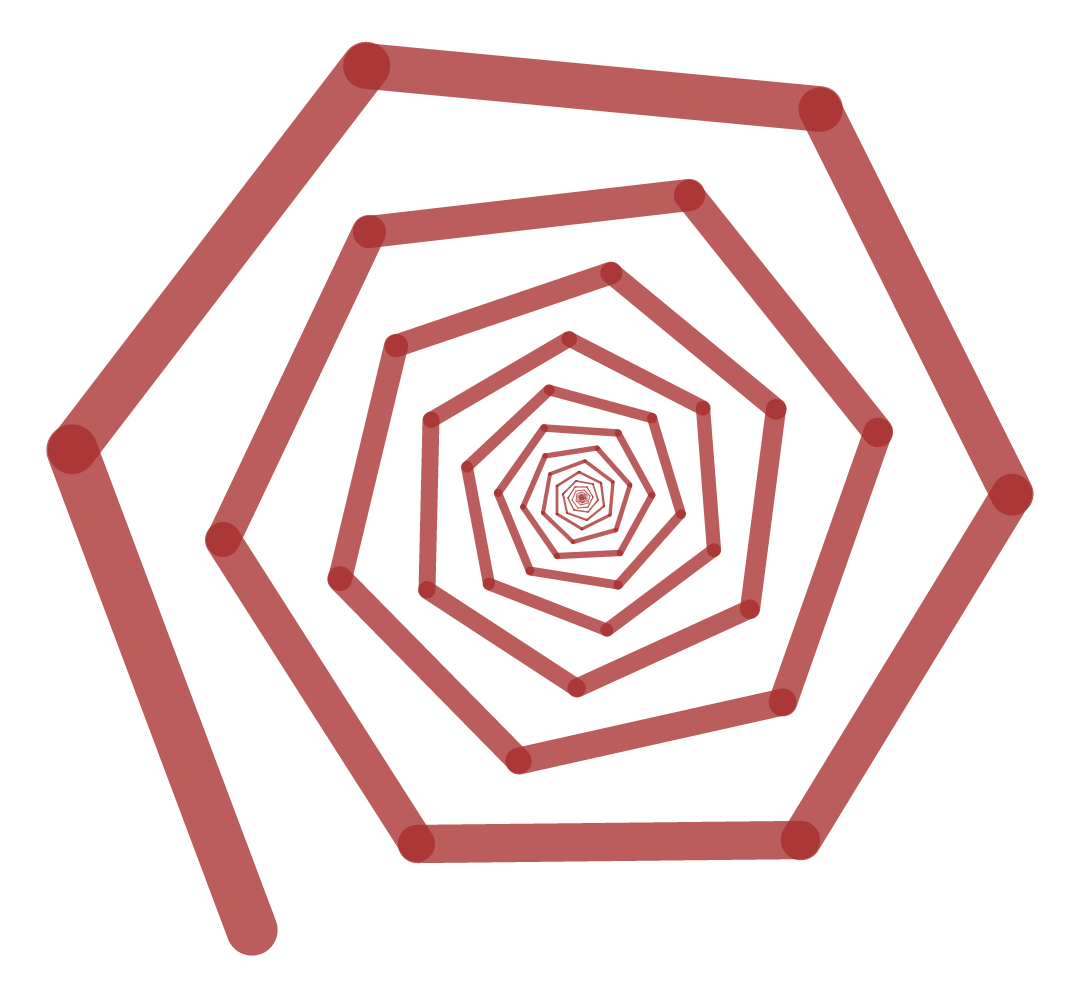
\includegraphics[width=0.24\textwidth]{img/Simple_Techniques/Spirals/spiral_simple_01.png}
            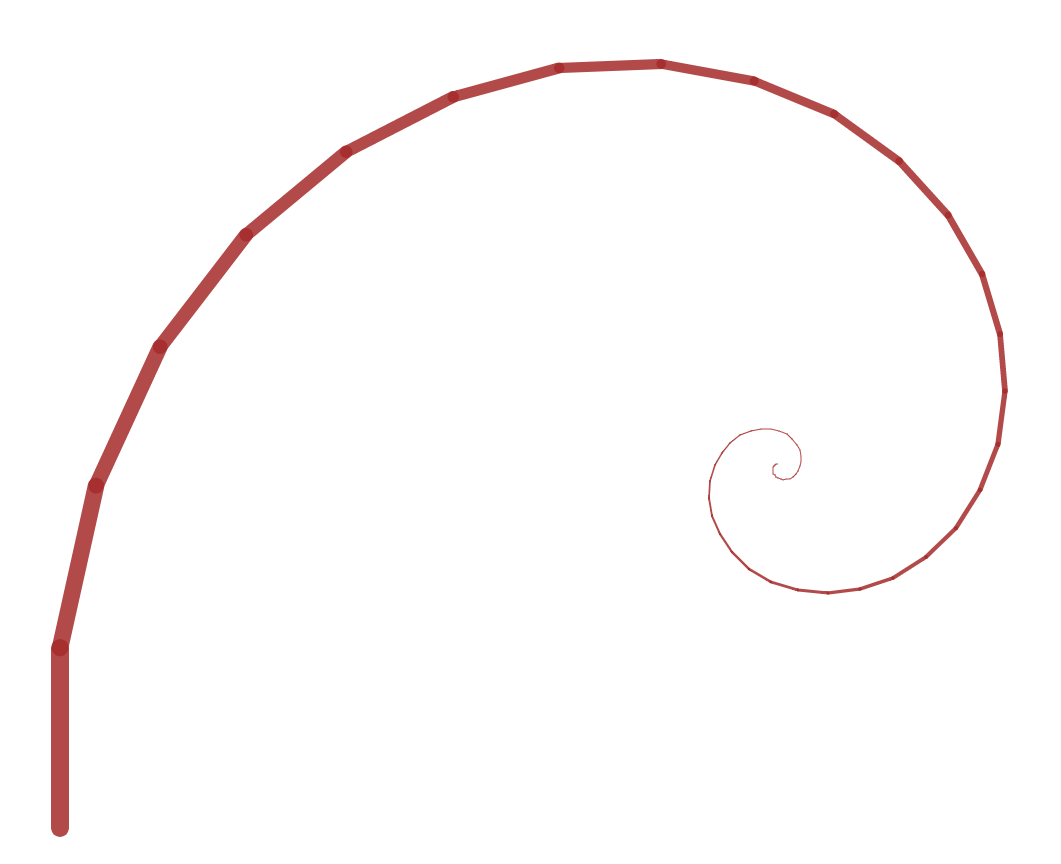
\includegraphics[width=0.24\textwidth]{img/Simple_Techniques/Spirals/spiral_simple_02.png}
            % 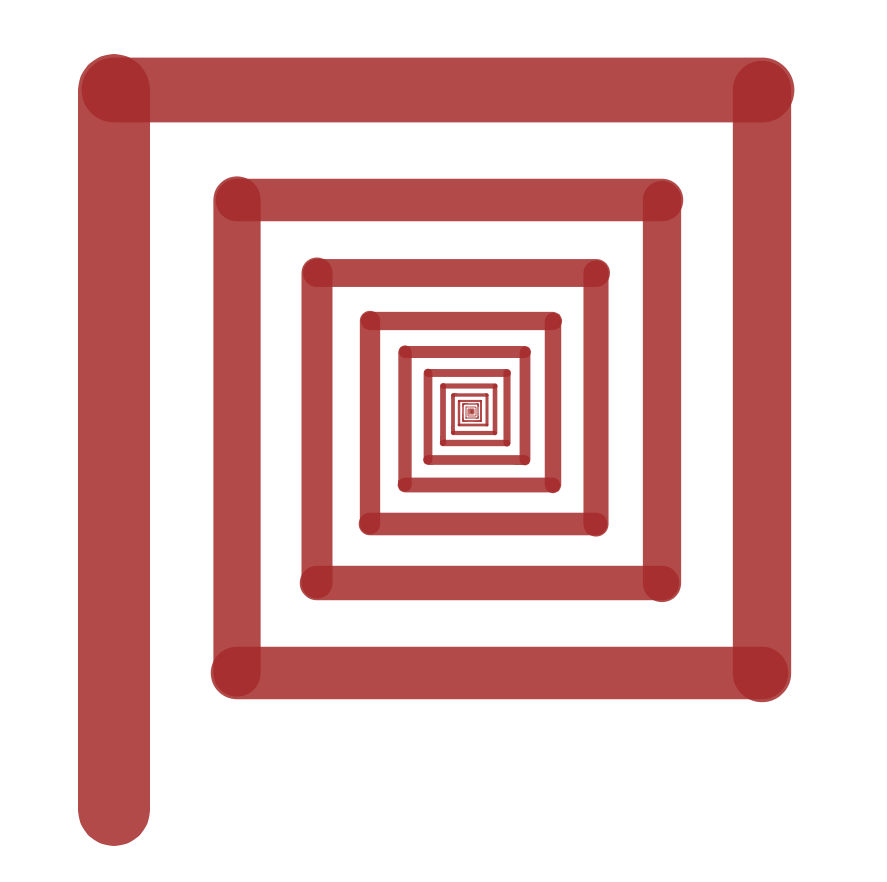
\includegraphics[width=0.24\textwidth]{img/Simple_Techniques/Spirals/spiral_simple_03.png}
            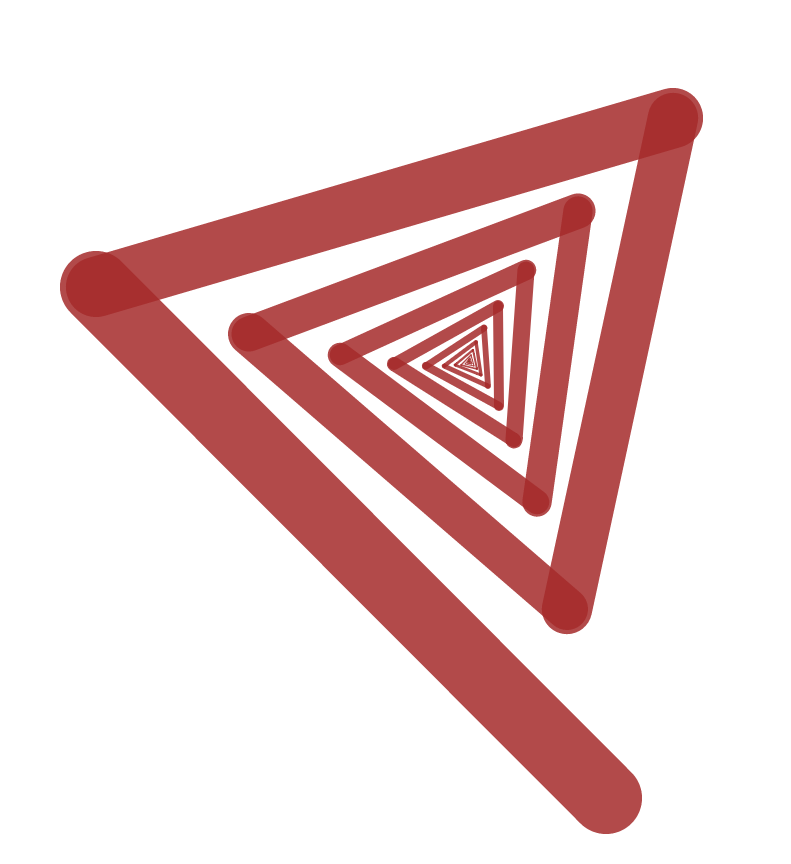
\includegraphics[width=0.24\textwidth]{img/Simple_Techniques/Spirals/spiral_simple_04.png}
            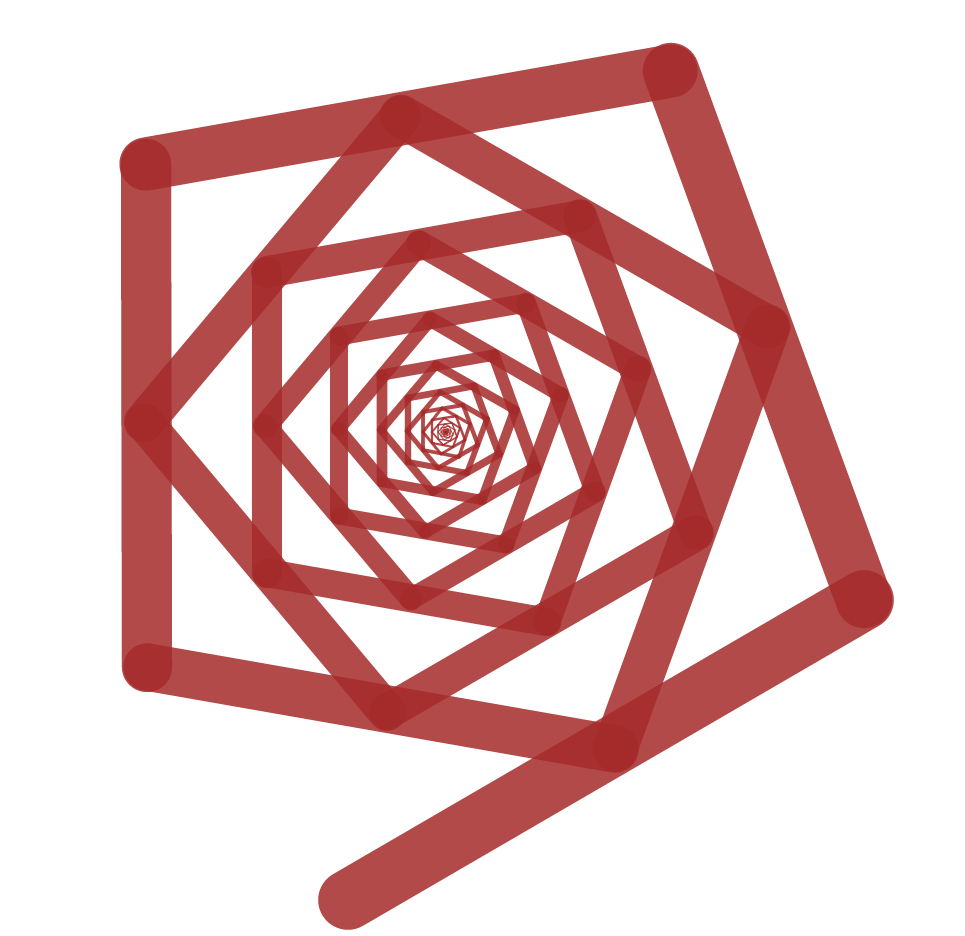
\includegraphics[width=0.24\textwidth]{img/Simple_Techniques/Spirals/spiral_simple_05.png}
        \end{figure}


        \FloatBarrier

        \subsubsection{Types of simple spirals}

            The most straightforward way to classify spirals is by the length of their recursive segment.
            Therefore, there are 3 type of spirals.
            The ones which were discussed earlier are the most common type --- \emph{convergent spiral}.
            Convergent spiral are spirals in which the length of the recursive segment is smaller than the length of the identity segment.
            Because of the aforementioned condition, convergent spirals always converge.

            \begin{figure}[ht]
                \centering
                \caption{\label{spiral_diver_01} An example of an divergent and a stationary spiral.}
                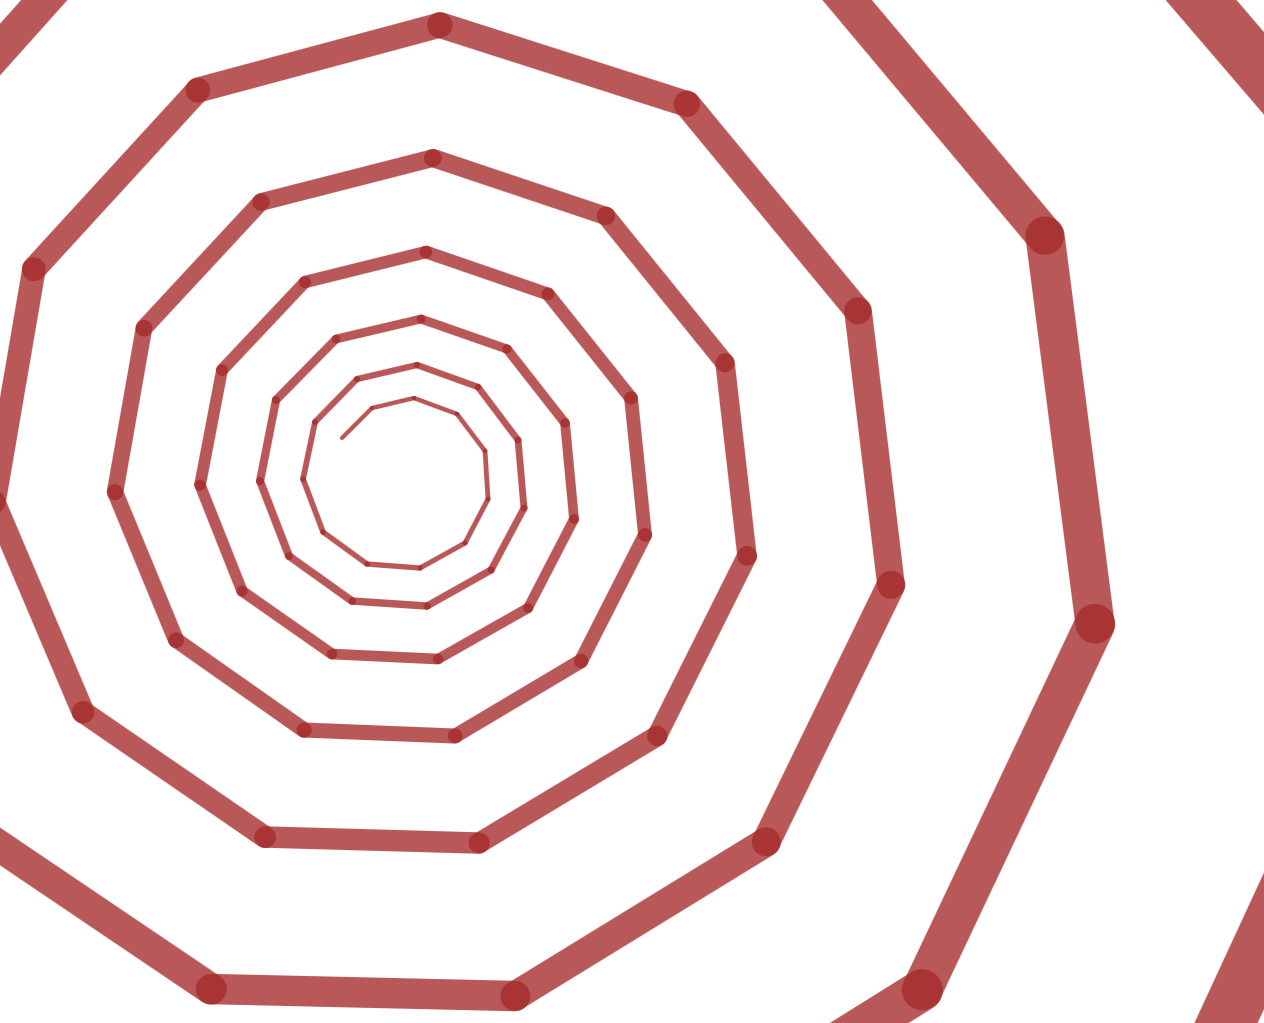
\includegraphics[height=0.2\textwidth]{img/Simple_Techniques/Spirals/spiral_diver_01.png}
                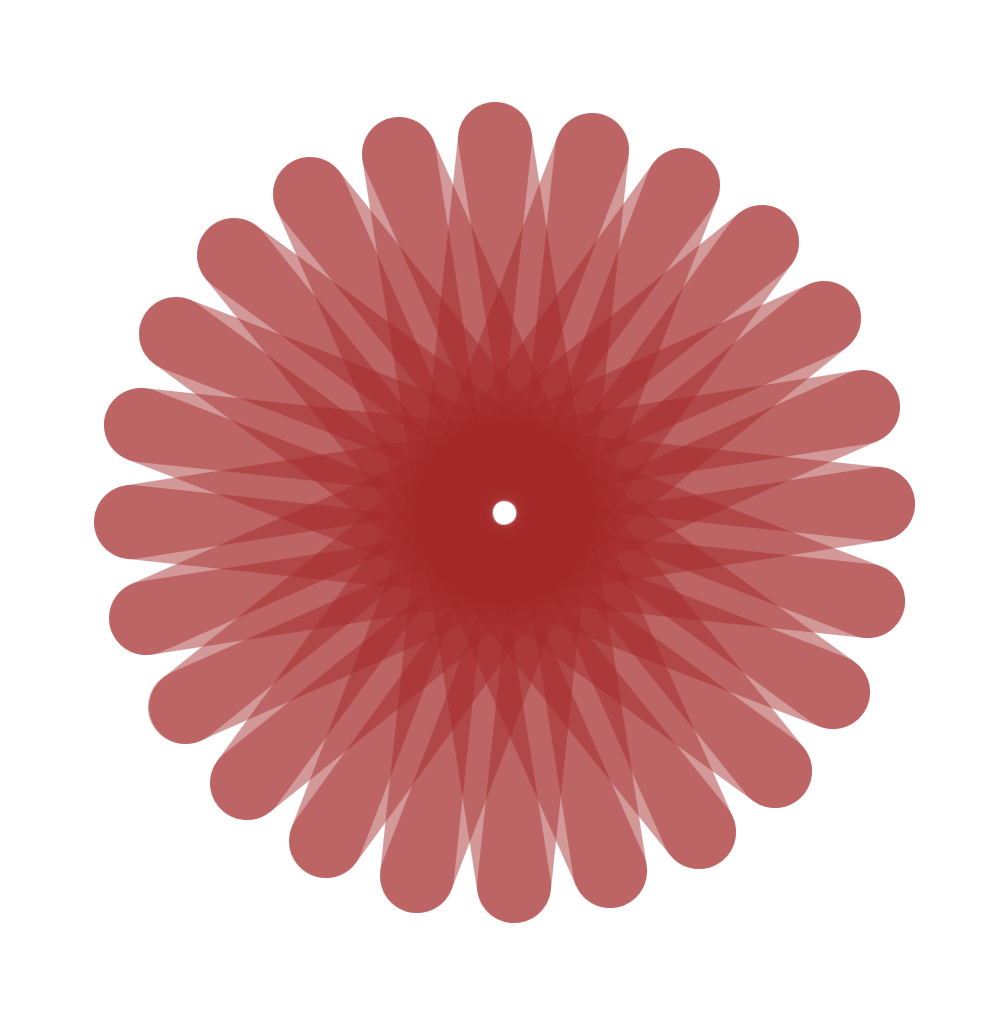
\includegraphics[height=0.2\textwidth]{img/Simple_Techniques/Spirals/spiral_diver_02.png}
            \end{figure}

            \FloatBarrier


            Besides this, there are of course two other types.
            There are divergent and stationary spirals.
            Usually divergent and stationary spirals are not as interesting as convergent ones, yet, they still can create beautiful figures, as shown in Figure~\ref{spiral_diver_01}.

            As a side note, the best method to create stationary spirals is by using the polar coordinates grid like in Figure~\ref{spiral_diver_setup_01}.
            In this way the length of the segments remain the same and the user has to change only the angle, which is trivial.

            \begin{figure}[ht]
                \centering
                \caption{\label{spiral_diver_setup_01} The setup of a stationary spiral.}
                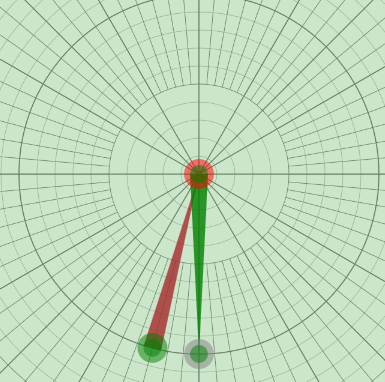
\includegraphics[height=0.3\textwidth]{img/Simple_Techniques/Spirals/spiral_diver_setup_01.png}
            \end{figure}

            \FloatBarrier

        \subsubsection{More interesting spirals}

            An interesting technique is to use two transformations in order to create a single spiral.
            The main one will go in the direction of the rotation of the spiral, as usual, but the second one will go in the opposed direction.
            In this way a zig-zag pattern can be observed.

            \begin{figure}[ht]
                \caption{\label{spiral_simple_02} A more interesting spiral setup.}
                \centering
                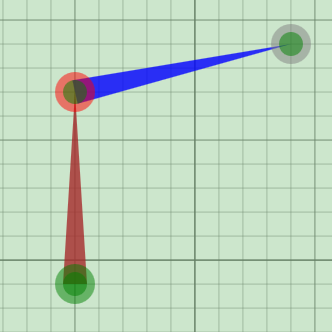
\includegraphics[height=0.3\textwidth]{img/Simple_Techniques/Spirals/spiral_set_02_01.png}
                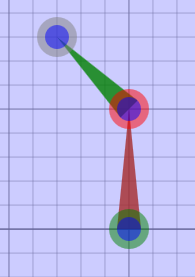
\includegraphics[height=0.3\textwidth]{img/Simple_Techniques/Spirals/spiral_set_02_02.png}
            \end{figure}

            \FloatBarrier

            As it can be observed, the green transformation has a quite long recursion segment.
            This will compensate for the fact that the blue transformation goes in the opposing direction.
            Figure~\ref{spiral_simple_03} shows how such spirals can look.
            One of the figures doesn't even look like a spiral (more like a zig-zagging straight path) but keeping the convention, it will be named like one.

            \begin{figure}[ht]
                \caption{\label{spiral_simple_03} More interesting spirals.}
                \centering
                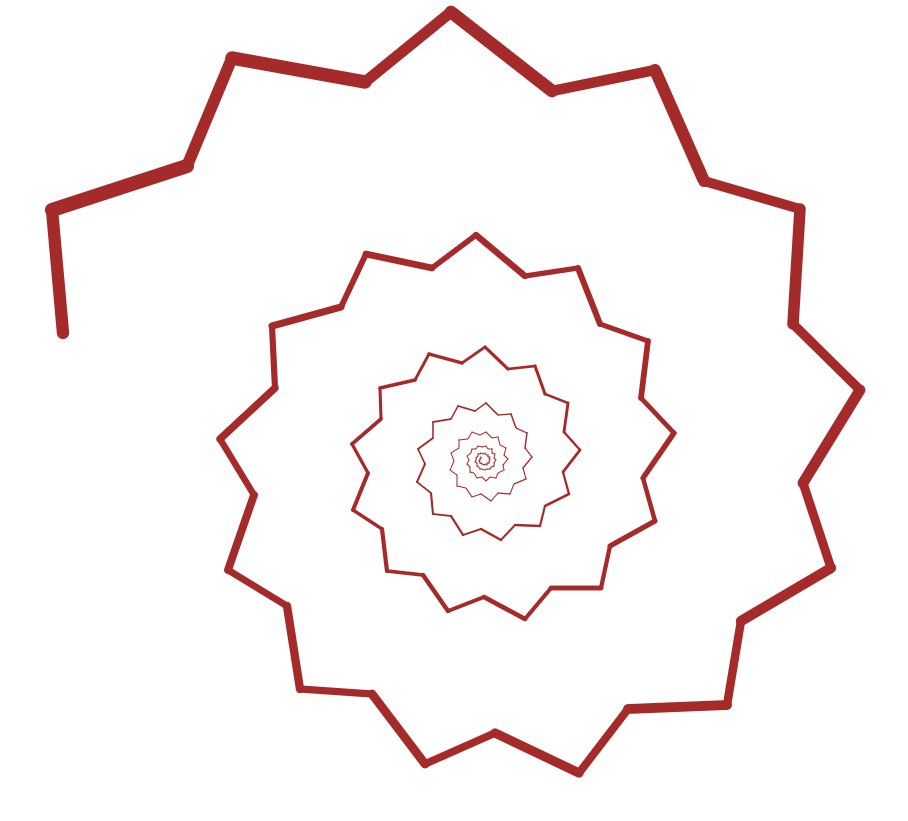
\includegraphics[height=0.2\textwidth]{img/Simple_Techniques/Spirals/spiral_04.png}
                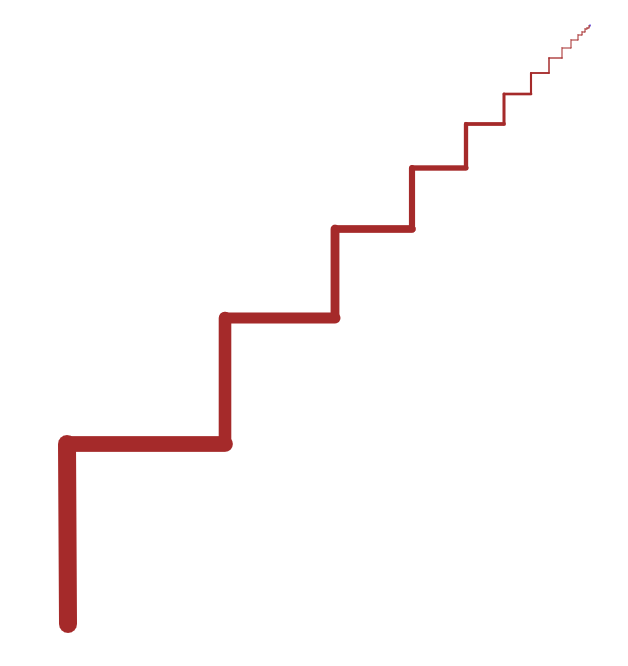
\includegraphics[height=0.2\textwidth]{img/Simple_Techniques/Spirals/spiral_05.png}
                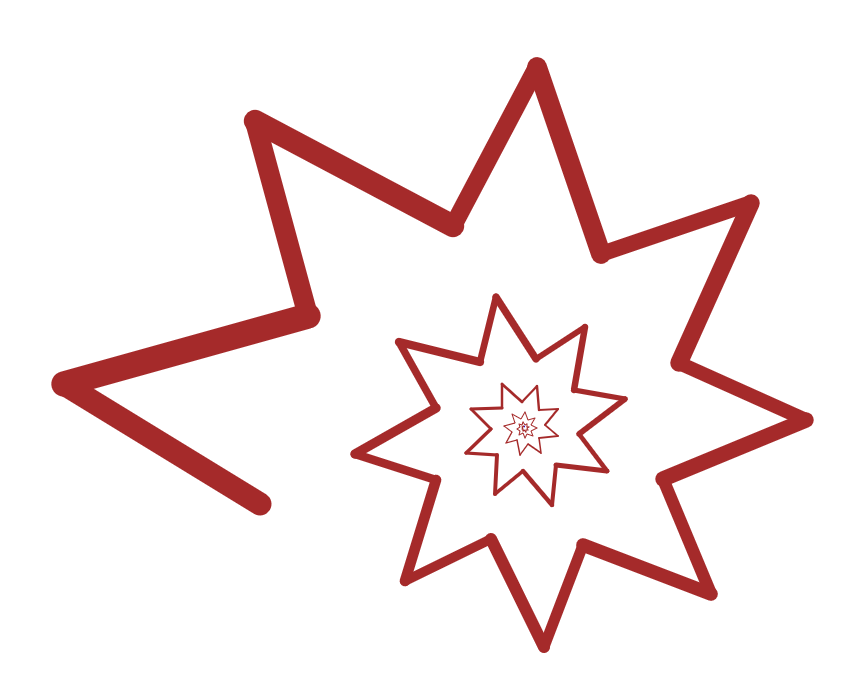
\includegraphics[height=0.2\textwidth]{img/Simple_Techniques/Spirals/spiral_06.png}
                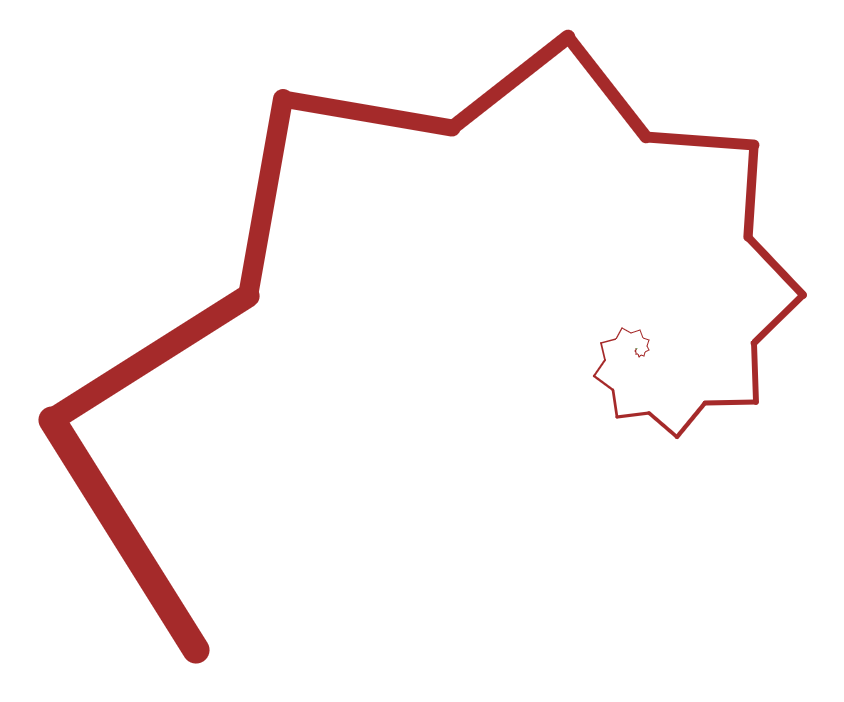
\includegraphics[height=0.2\textwidth]{img/Simple_Techniques/Spirals/spiral_07.png}
            \end{figure}

            \FloatBarrier

    \subsection{Simple Trees}

        By \emph{Tree} I mean not only transformations that resemble trees but also any figure in which a tree-like structure can be distinguished.
        Just as spirals trees can be classified in convergent, divergent and stationary, yet I will only discuss convergent trees since the other two type do not have very interesting features.

        \subsubsection{Trees with two branches}
            Let's begin by creating a figure that resembles the Pythagoras Tree.
            For this particular tree I switched to Polar Coordinates grid so that I could put the branches at exactly 120\textdegree degrees.

            \begin{figure}[ht] 
                \caption{\label{simple_tree_set_01} A geometric tree setup and its corresponding fractal.}
                \centering
                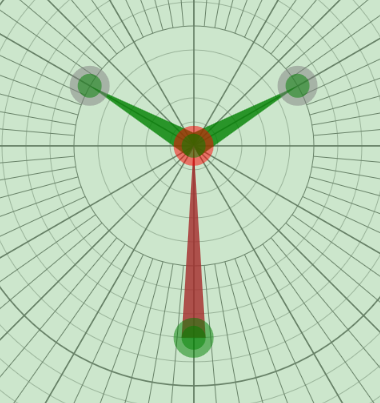
\includegraphics[height=0.3\textwidth]{img/Simple_Techniques/Trees/tree_set_01.png}
                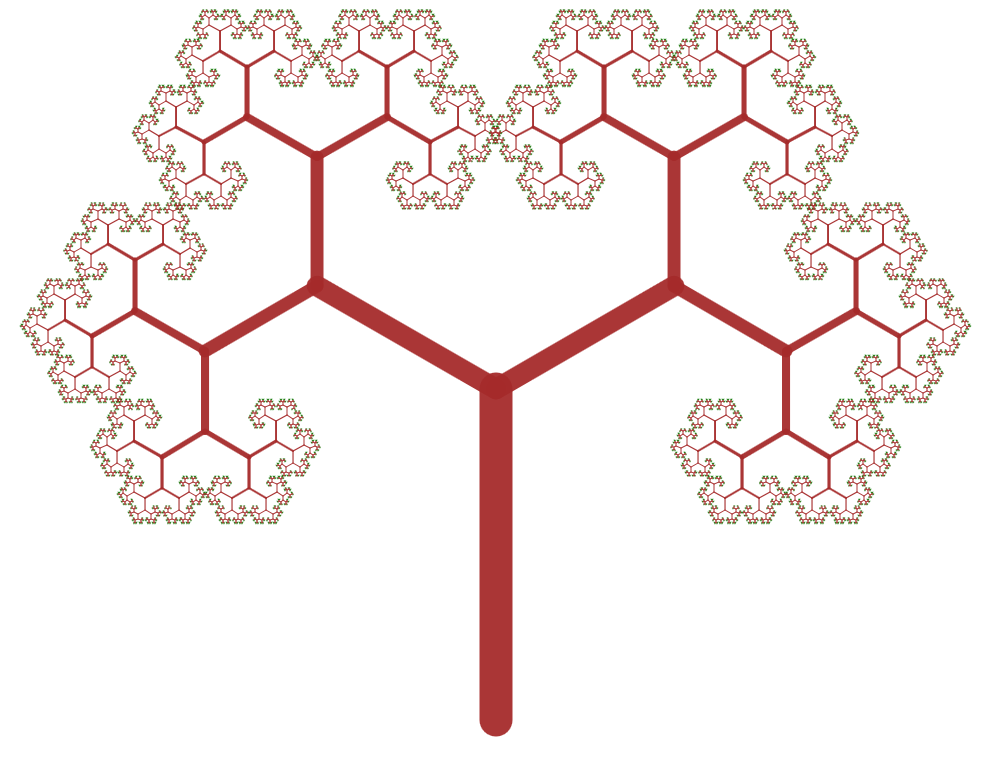
\includegraphics[height=0.4\textwidth]{img/Simple_Techniques/Trees/tree_01.png}
                
            \end{figure}

            Trees look like a natural progression from spirals. 
            Spirals where bound to use just one recursion \emph{branch} whereas trees can use two, or more, as we'll see further.

            Figure~\ref{simple_tree_02} shows some possible types of trees. 

            \begin{figure}[ht]
                \caption{\label{simple_tree_02} Some trees.}
                \centering
                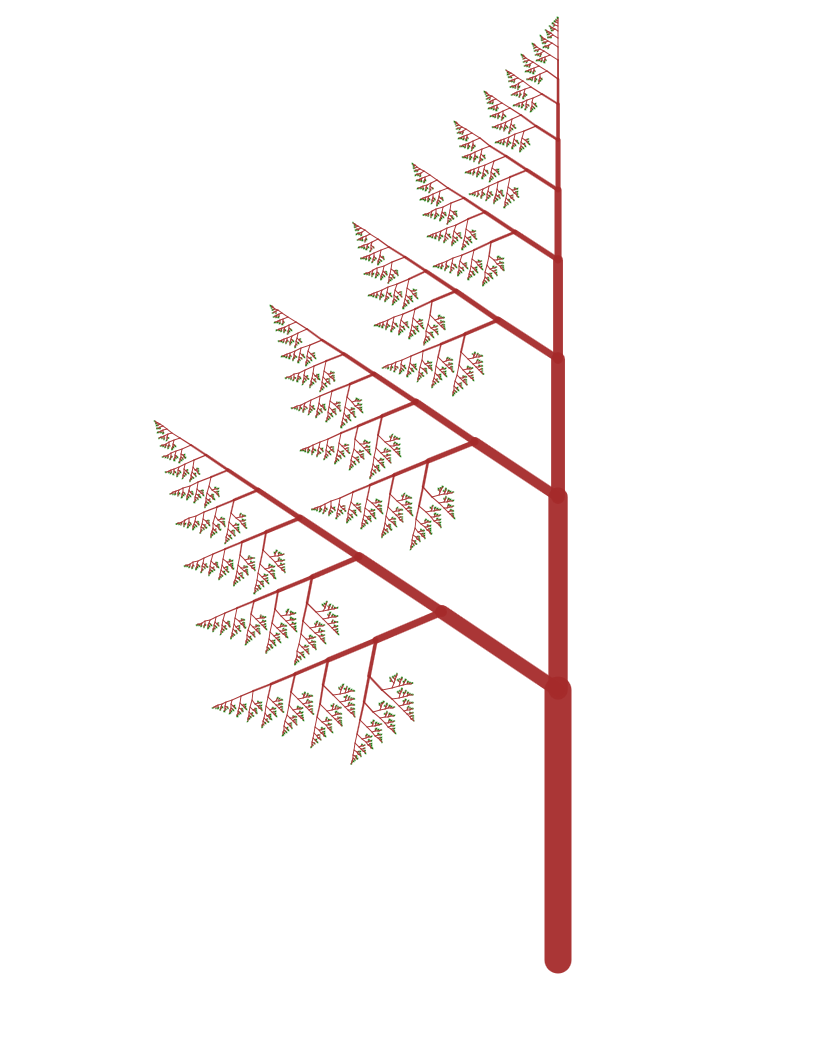
\includegraphics[width=0.27\textwidth]{img/Simple_Techniques/Trees/tree_02.png}
                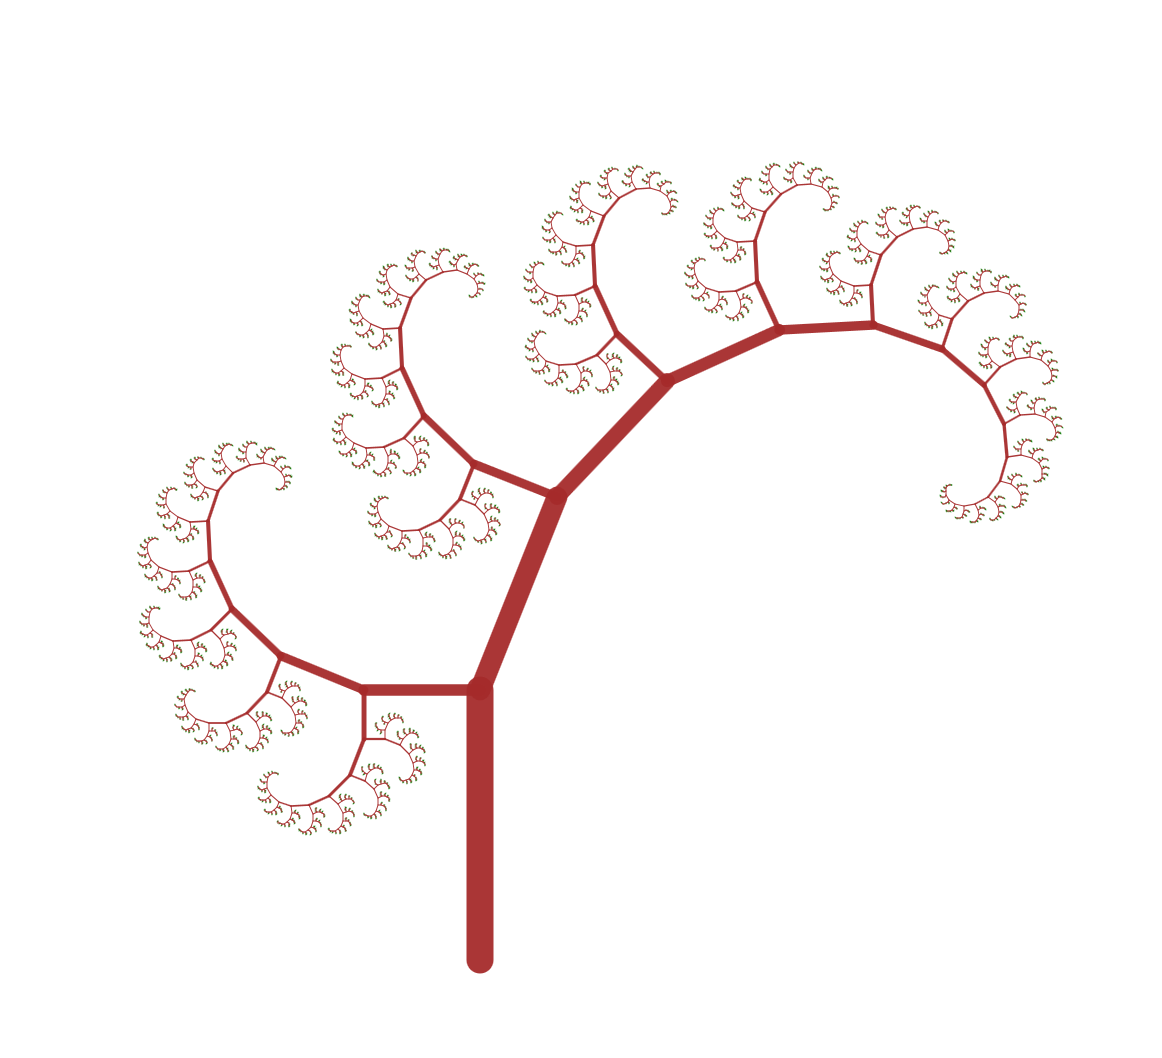
\includegraphics[width=0.27\textwidth]{img/Simple_Techniques/Trees/tree_03.png}
                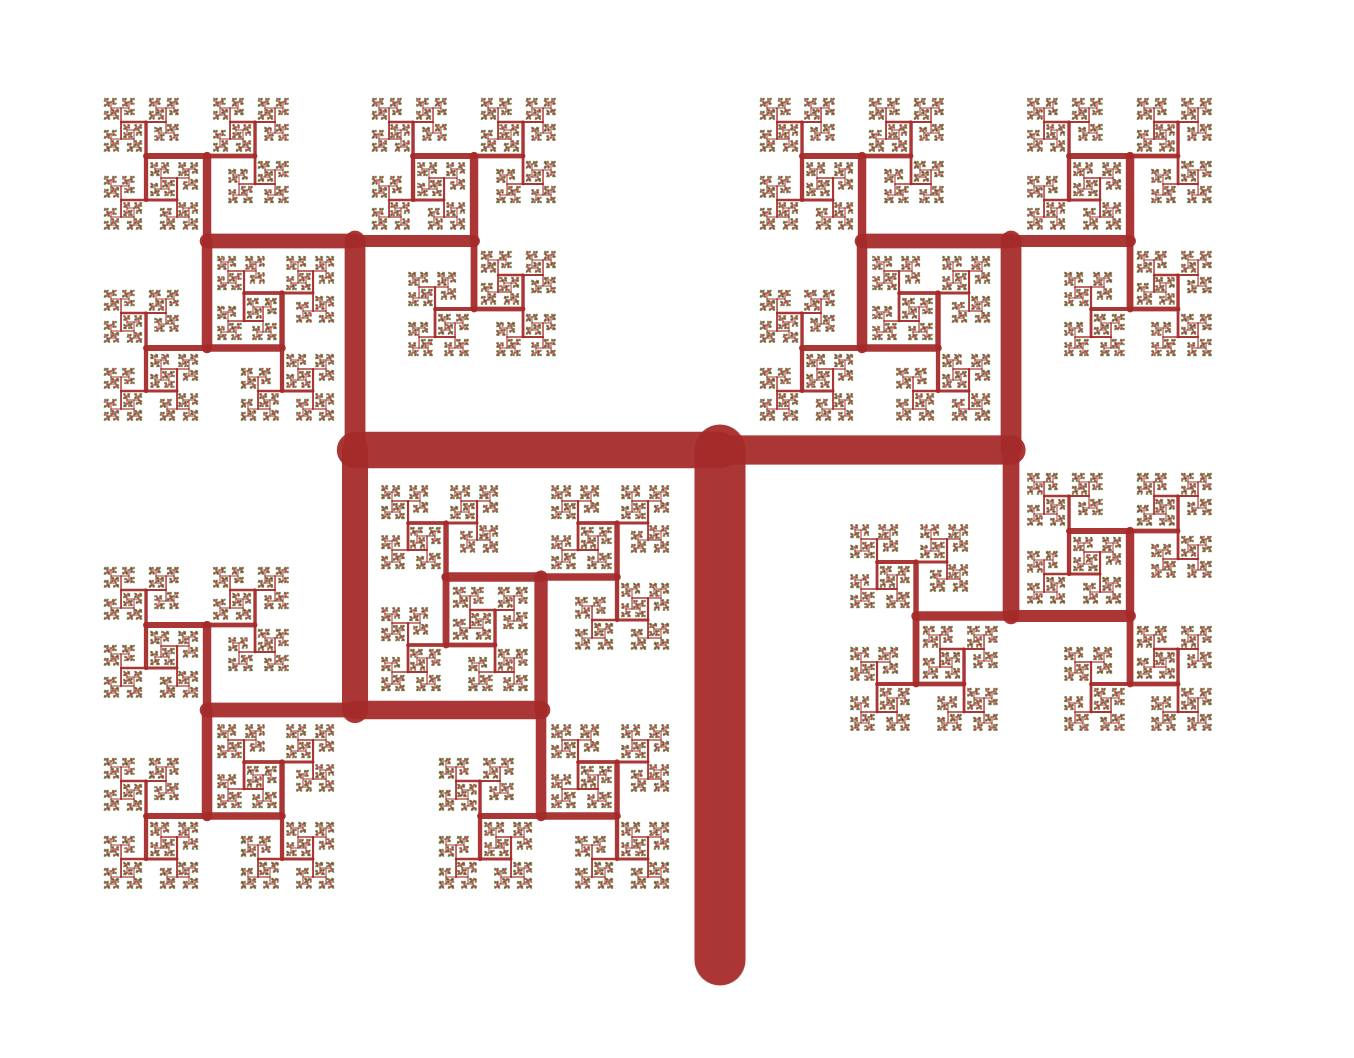
\includegraphics[width=0.27\textwidth]{img/Simple_Techniques/Trees/tree_04.png}
                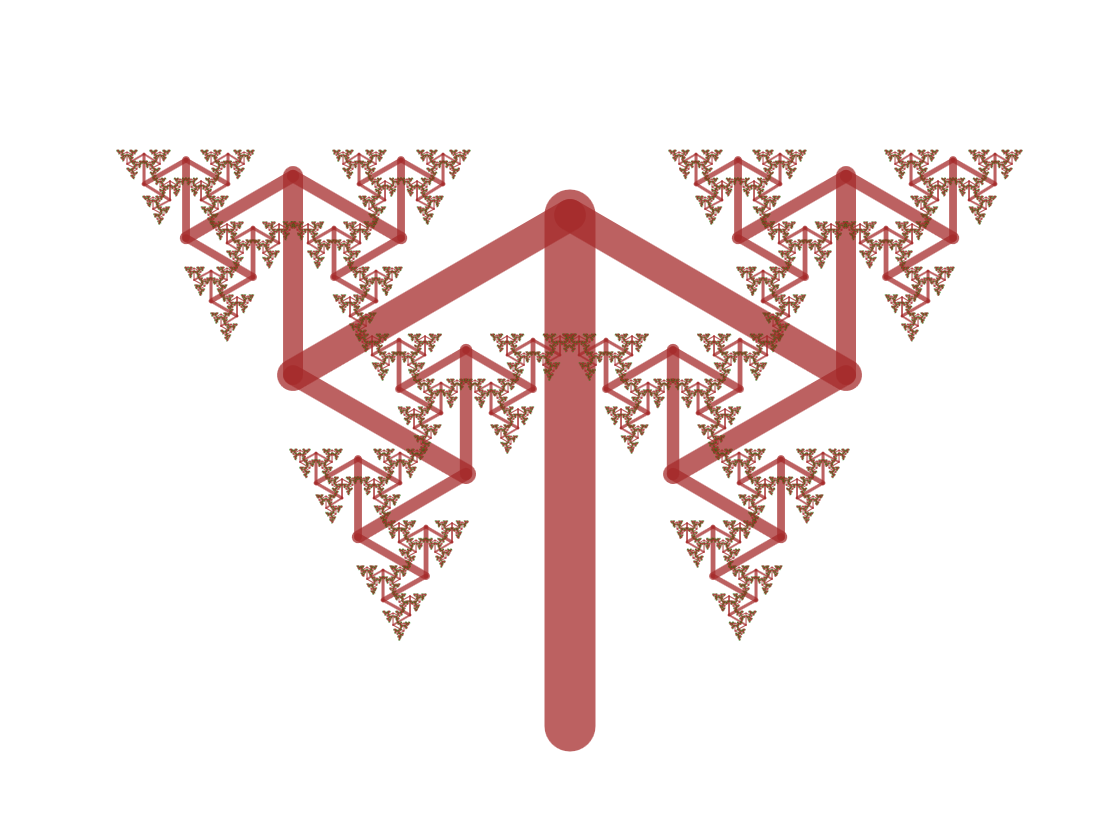
\includegraphics[width=0.27\textwidth]{img/Simple_Techniques/Trees/tree_05.png}
                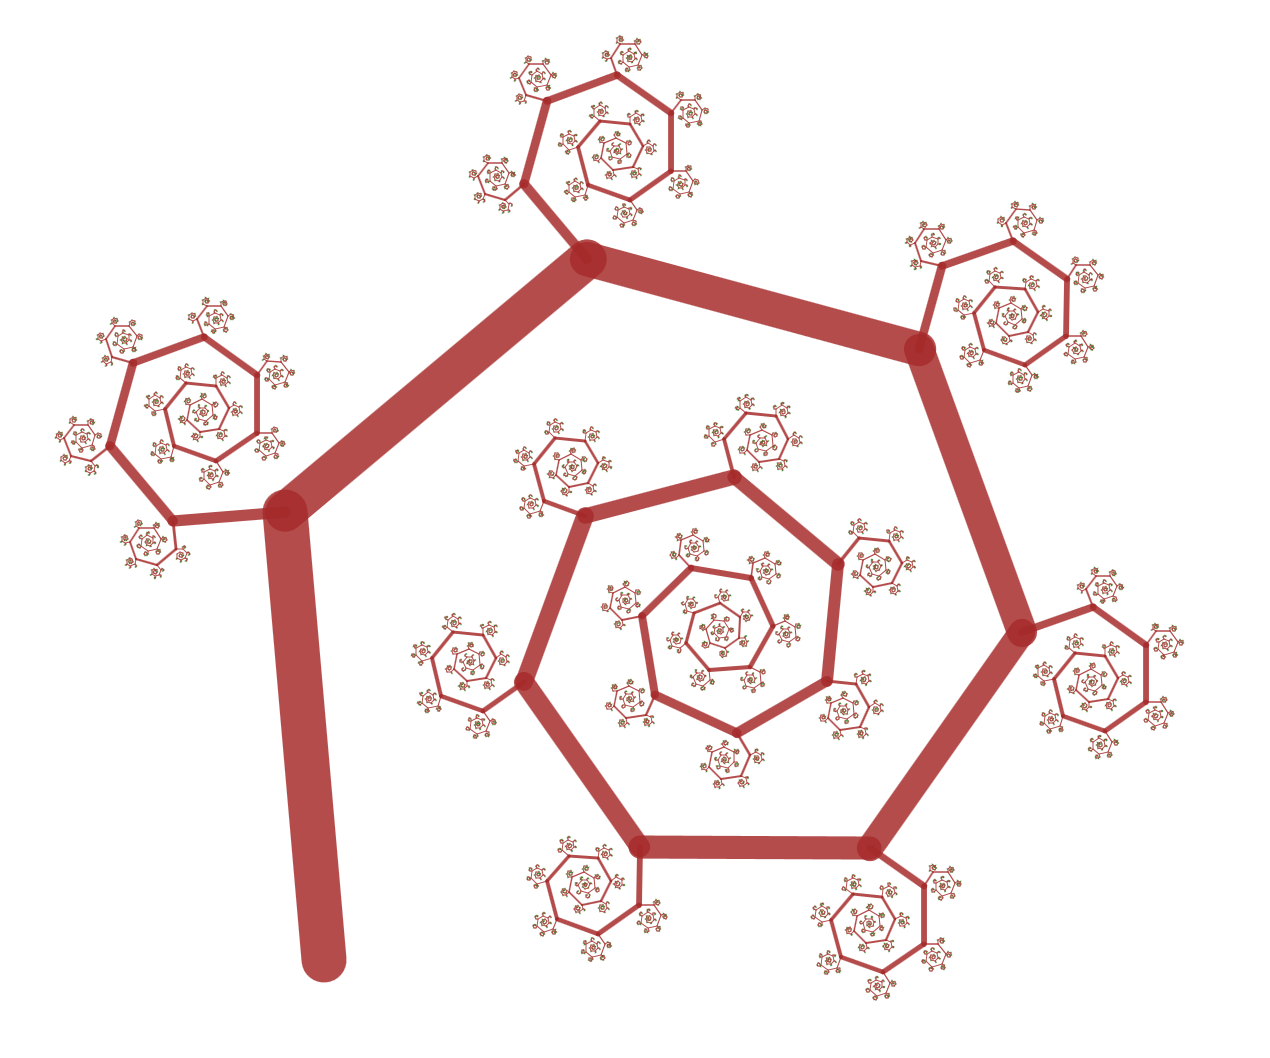
\includegraphics[width=0.27\textwidth]{img/Simple_Techniques/Trees/tree_06.png}
                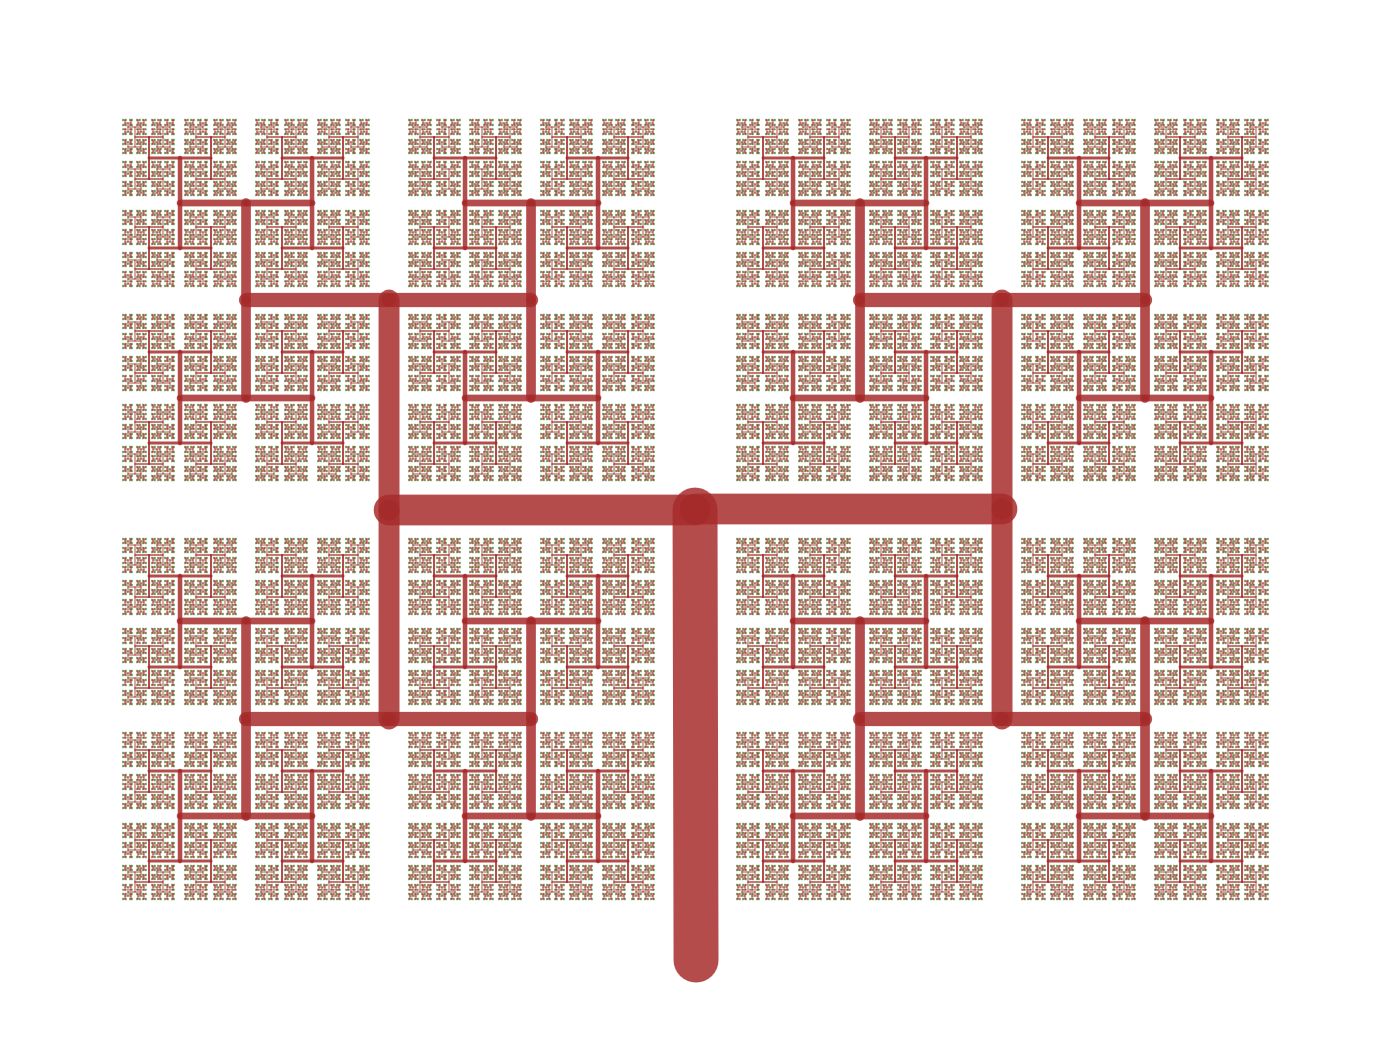
\includegraphics[width=0.27\textwidth]{img/Simple_Techniques/Trees/tree_07.png}                
            \end{figure}

            \FloatBarrier

            Some of these trees start to degenerate to spirals with an added node. 
            I will come back to these types of spirals later.

        \subsubsection{Trees with multiple branches}

            Figure~\ref{simple_tree_03} shows some examples of trees with multiple branches.
            Usually having many branches results in getting a clustered fractal so choosing a good transformation is very important.
            

            \begin{figure}[ht]
                \caption{\label{simple_tree_03} Trees with several branches.}
                \centering
                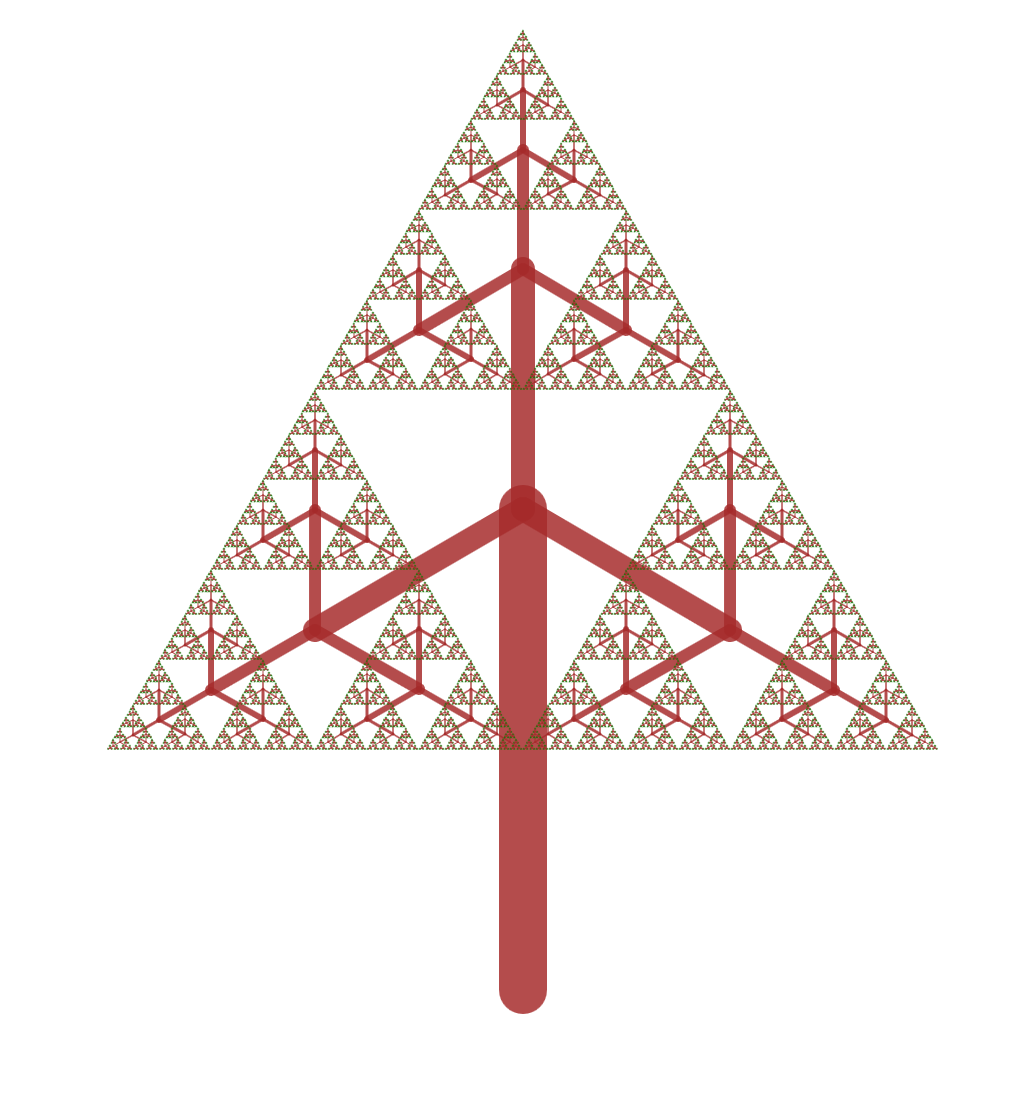
\includegraphics[width=0.32\textwidth]{img/Simple_Techniques/Trees/tree_08.png}
                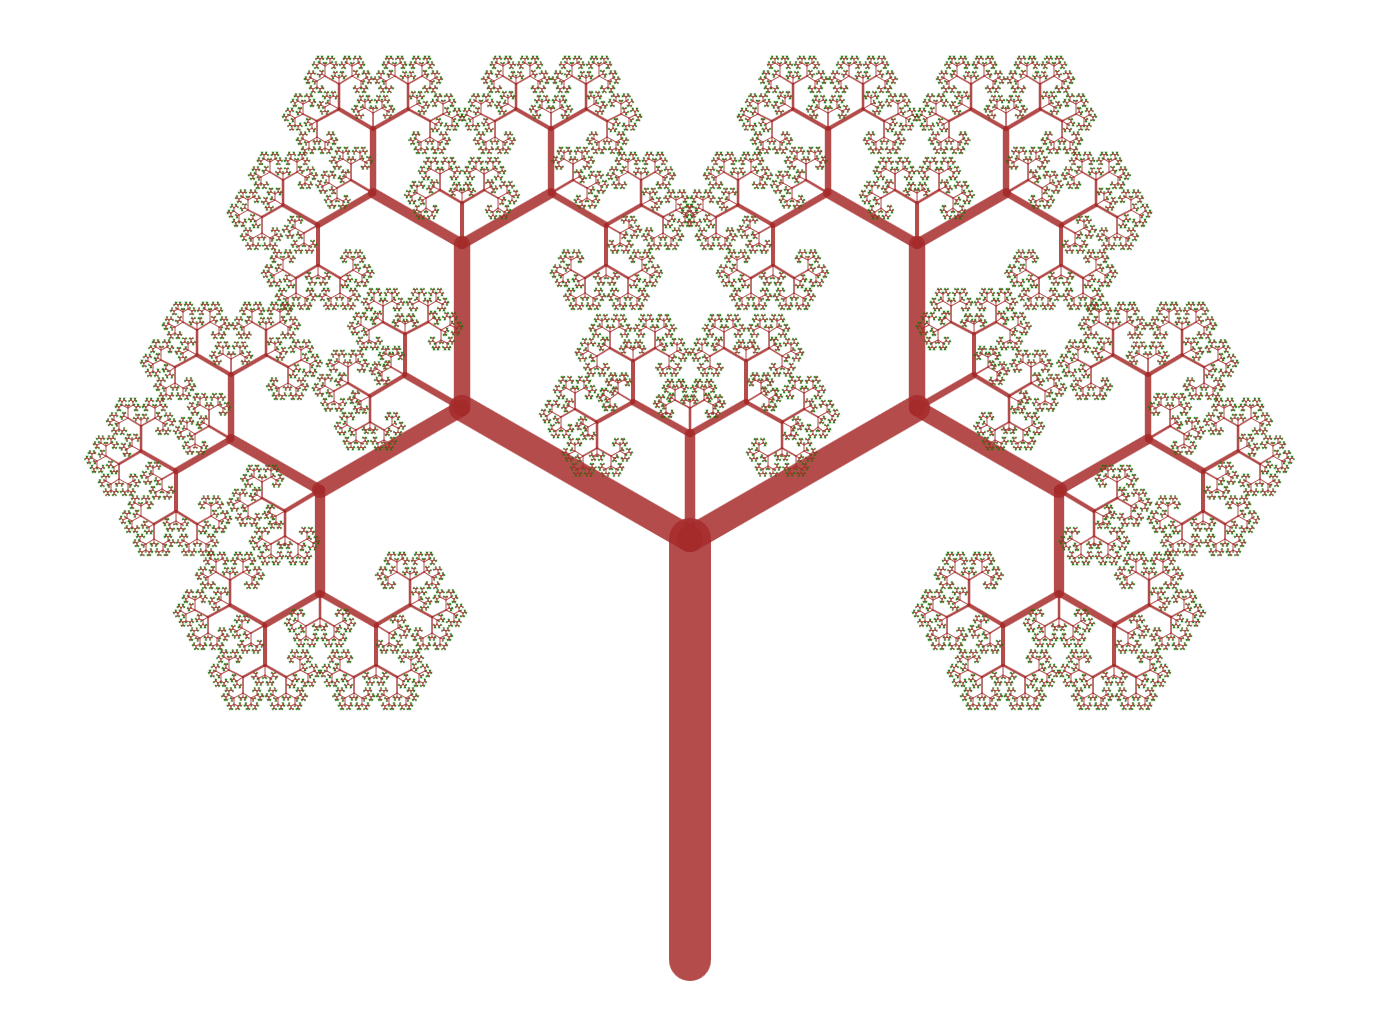
\includegraphics[width=0.32\textwidth]{img/Simple_Techniques/Trees/tree_09.png}
                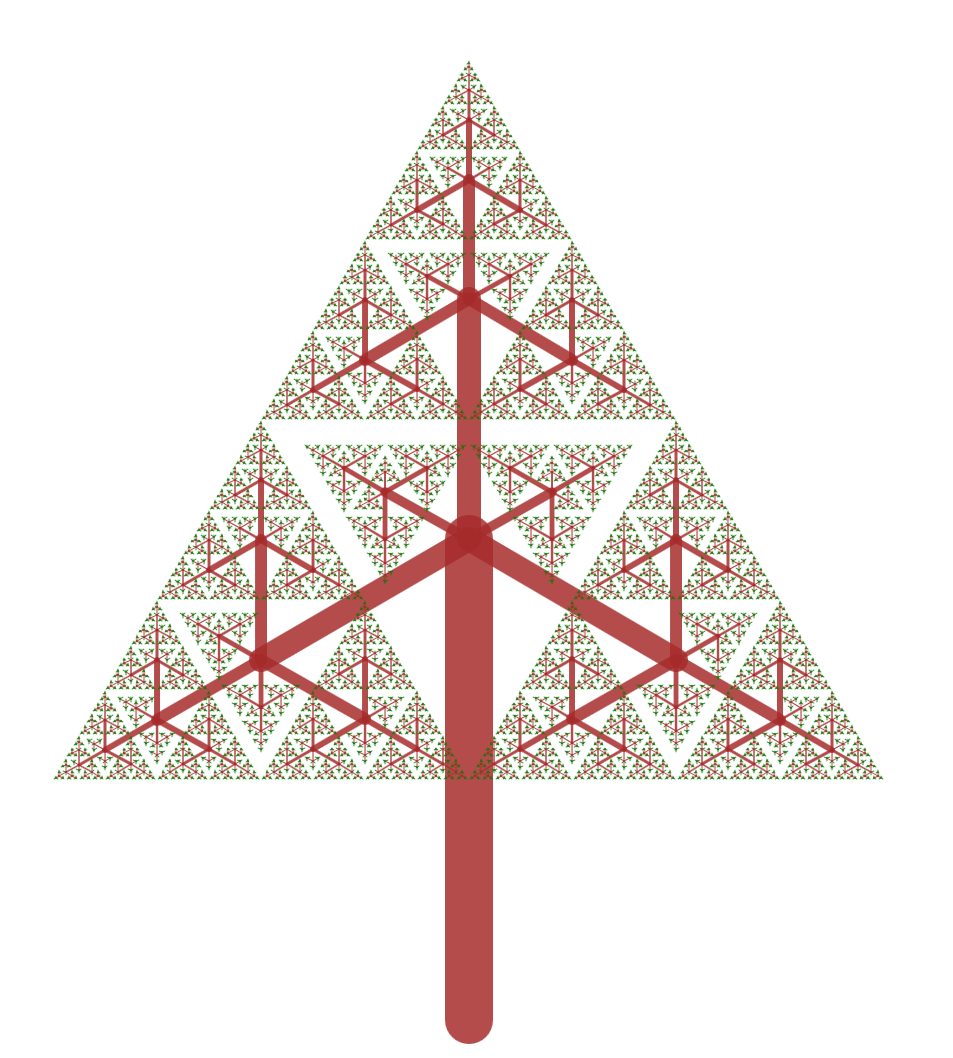
\includegraphics[width=0.32\textwidth]{img/Simple_Techniques/Trees/tree_10.png}             
            \end{figure}

            \FloatBarrier

        \subsubsection{Trees with multiple transformations}

            A much more interesting progression from simple trees is to use different transformations that call each other, just like in the beginning of the paper.

            \begin{figure}[ht]
                \caption{\label{simple_tree_set_02} Setup of a tree with two transformations.}
                \centering
                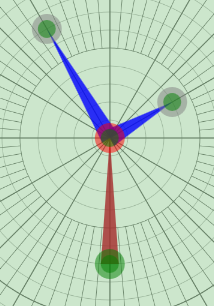
\includegraphics[height=0.3\textwidth]{img/Simple_Techniques/Trees/tree_set_02.png}
                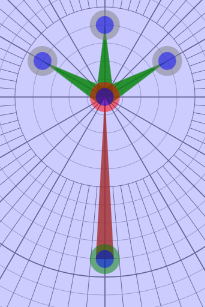
\includegraphics[height=0.3\textwidth]{img/Simple_Techniques/Trees/tree_set_03.png}  
                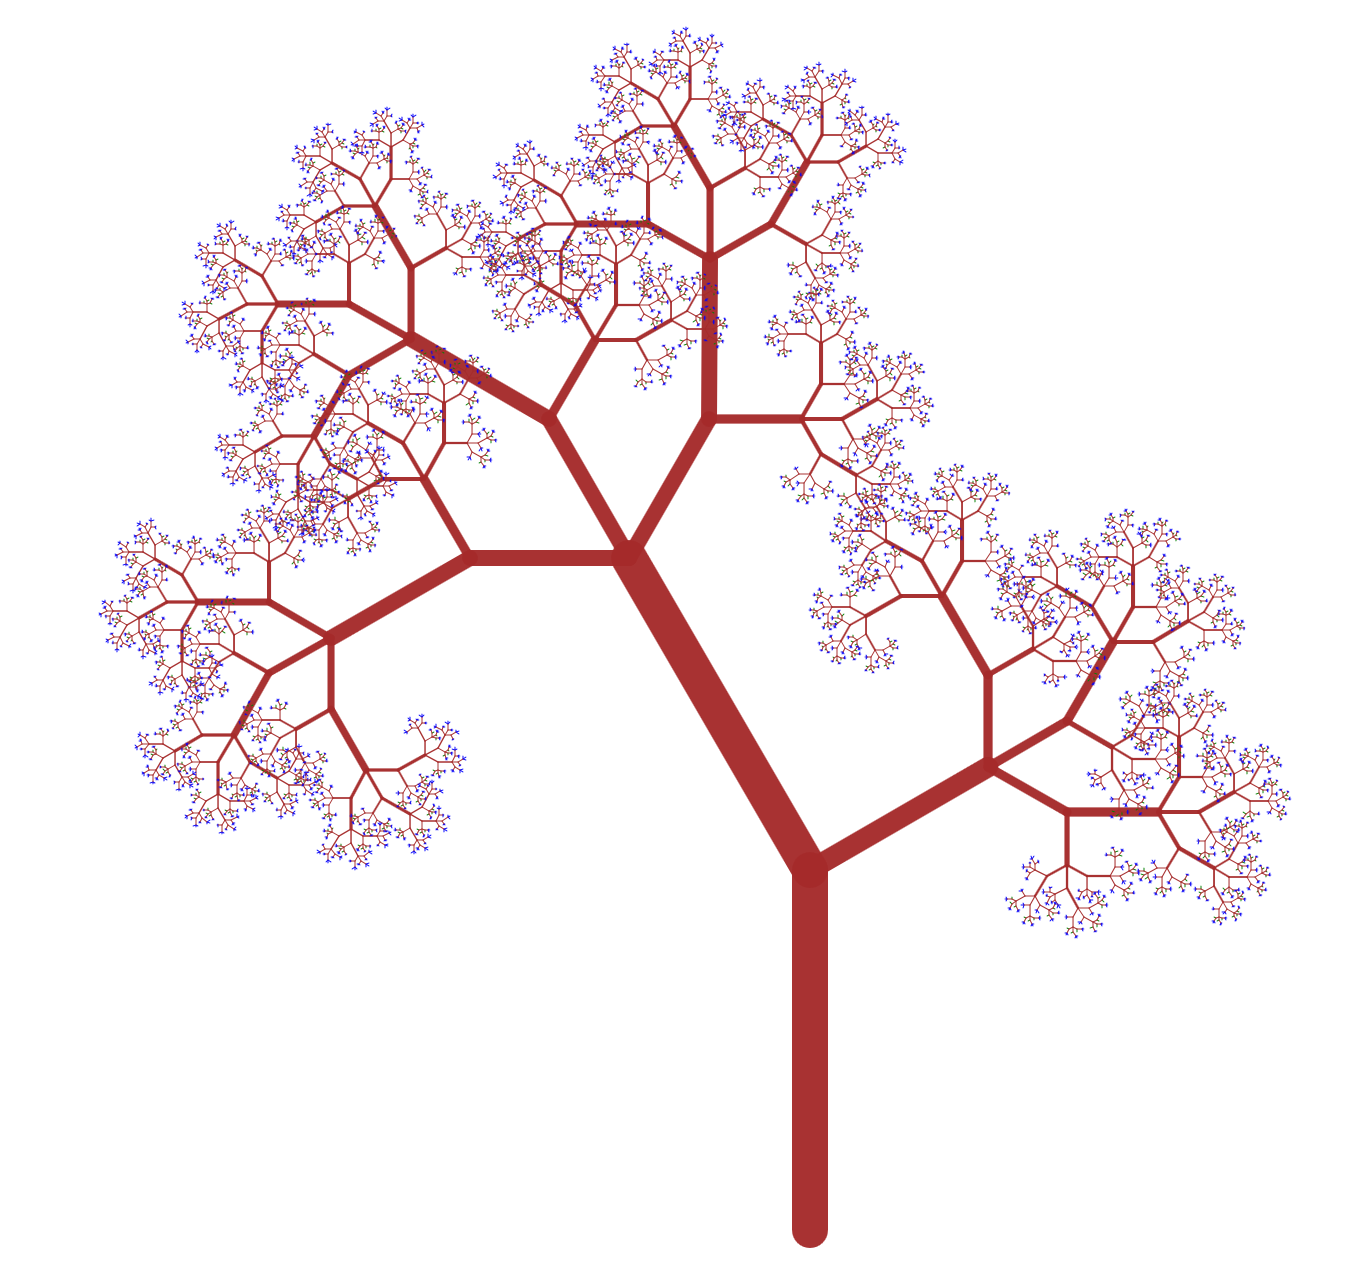
\includegraphics[width=0.6\textwidth]{img/Simple_Techniques/Trees/tree_12.png}          
            \end{figure}

            \FloatBarrier

            The reader should experiment and see whether he or she can find interesting types of trees using just these simple techniques.

    \subsection{Unconnected figures}
        Until now every transformation implied some kind of connection between segments.
        This is not necessary.
        We can easily create transformations without connections.
        Understanding the mathematical reasoning behind these type of transformations is very important.
        
        Let's start with two adjacent segment, which are not connected to the start nor the end point.
        Figure~\ref{simple_un_line_01} shows the setup.
        The progression shows how the lines evolve.

        \begin{figure}[H]
            \caption{\label{simple_un_line_01} Two segments.}
            \centering
            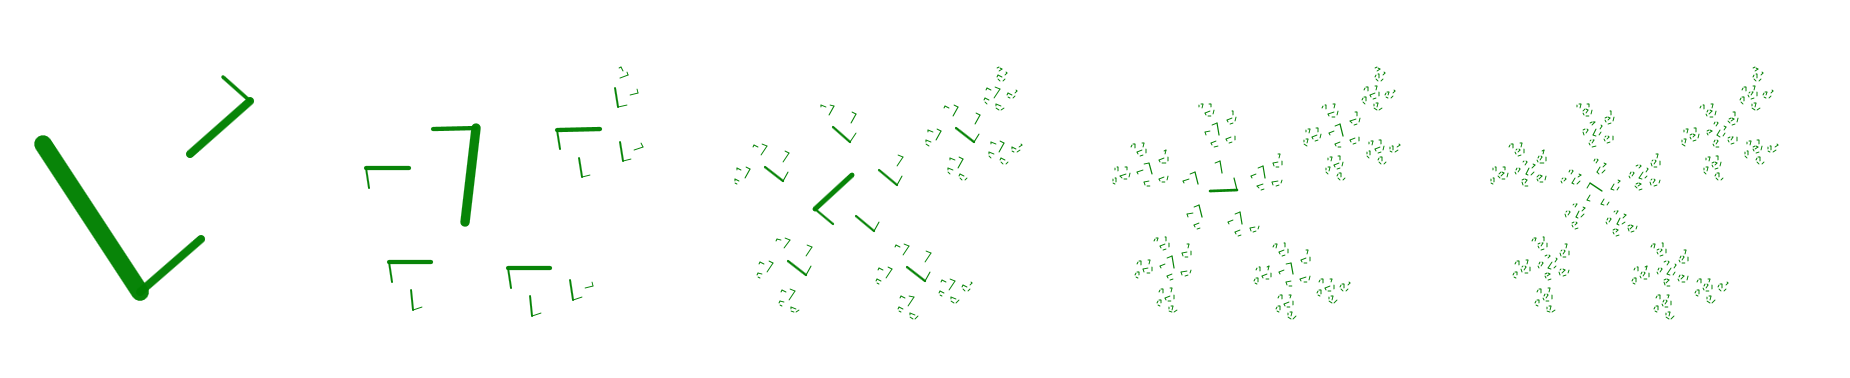
\includegraphics[width=1.0\textwidth]{img/Simple_Techniques/Unconnect/simple_un_lines_01.png}         
        \end{figure}

        The reasoning behind these transformations may seem rather obscure so let's go through it step by step.
        We start with a segment with the direction showed by the arrow.
        The transformation is superimposed (Fig.~\ref{simple_un_line_exp_01}).

        \begin{figure}[H]
            \caption{\label{simple_un_line_exp_01} The transformation step by step.}
            \centering
            \subcaptionbox{}[0.3\textwidth]
                {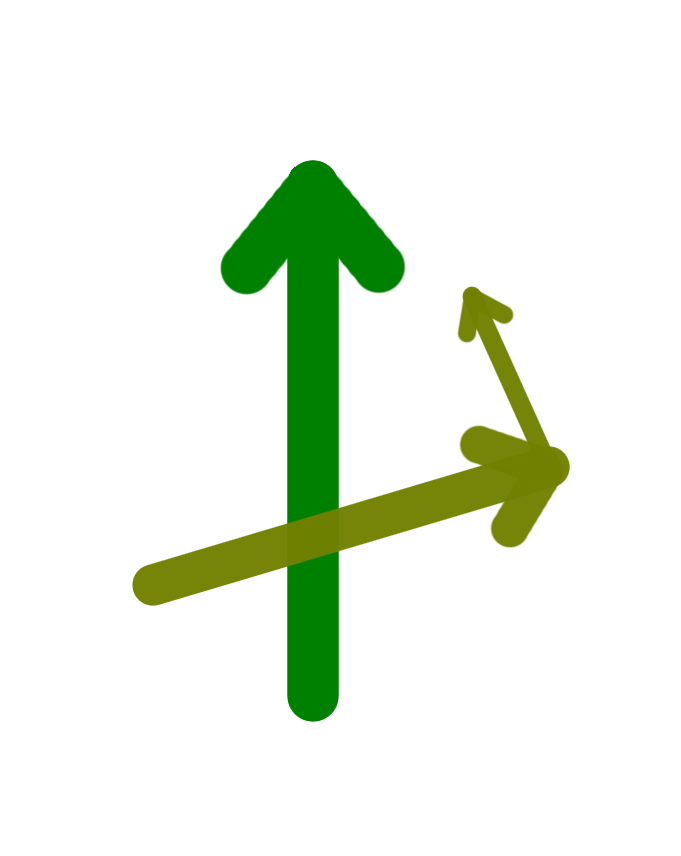
\includegraphics[height=0.3\textwidth]{img/Simple_Techniques/Unconnect/simple_line_exp_01.png}}
            ~
            \subcaptionbox{}[0.3\textwidth]
                {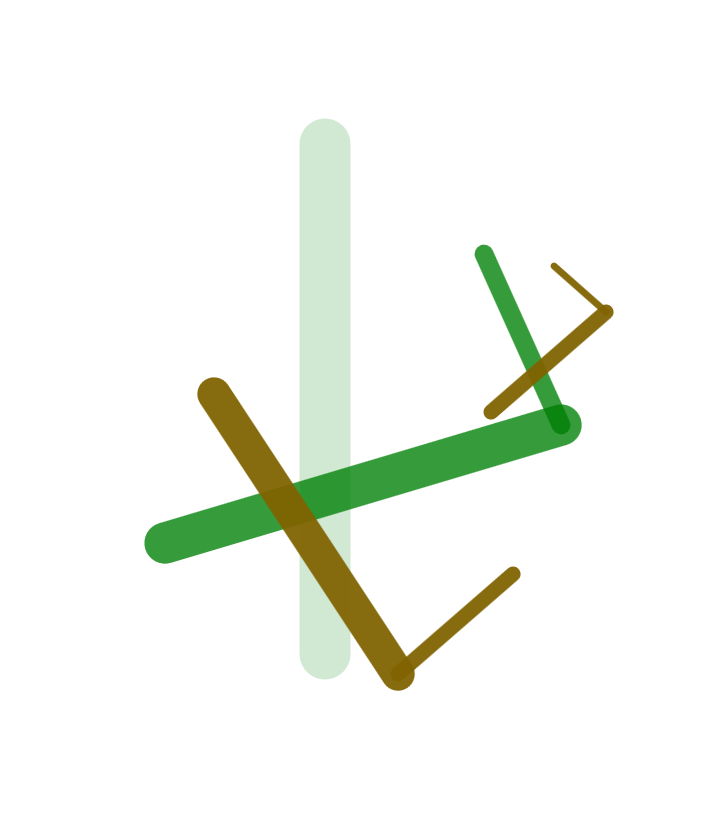
\includegraphics[height=0.3\textwidth]{img/Simple_Techniques/Unconnect/simple_line_exp_02.png}}
        \end{figure}
        \FloatBarrier

        Now, it should be clear how the mechanics of the transformation works.
        The arrows are very important, changing the direction of the arrow, usually, completely changes the visual aspect of the figure.

        A major problem with unconnected transformations is that they can diverge to 
            figures that are hard to observe since they are composed from very small parts.
        It is possible to create unconnected transformation with only one recursing segment but the behavior is trivial, 
            so the minimum segments for constructing an unconnected transformation (and actually any type of transformation) is two.

        When it comes to unconnected transformations the result is usually quite unexpected.
        It is hard to guess the final figure just by looking at the transformation.
        Figure~\ref{simple_un_triangle_01} shows an example.

        Sometimes, especially when dealing with unconnected transformations it is best to not iterate very deep.
        For example, in fig.~\ref{simple_un_quad_01} the iteration level is just 5.
        Also observe how unexpected the result is comparing to the setup.
        Some special cases of unconnected transformation will be discussed in further chapters.

        \begin{figure}[ht]
            \caption{\label{simple_un_triangle_01} A unconnected transformation with a triangle}
            \centering
            \subcaptionbox{}[0.2\textwidth]
                {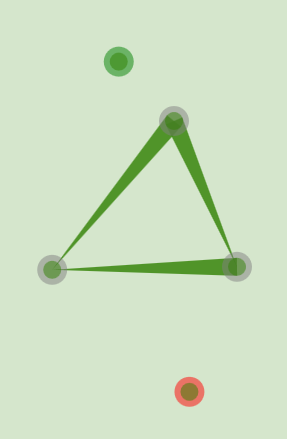
\includegraphics[width=0.2\textwidth]{img/Simple_Techniques/Unconnect/simple_un_setup_triangle_01.png}}
            \subcaptionbox{}[0.7\textwidth]
                {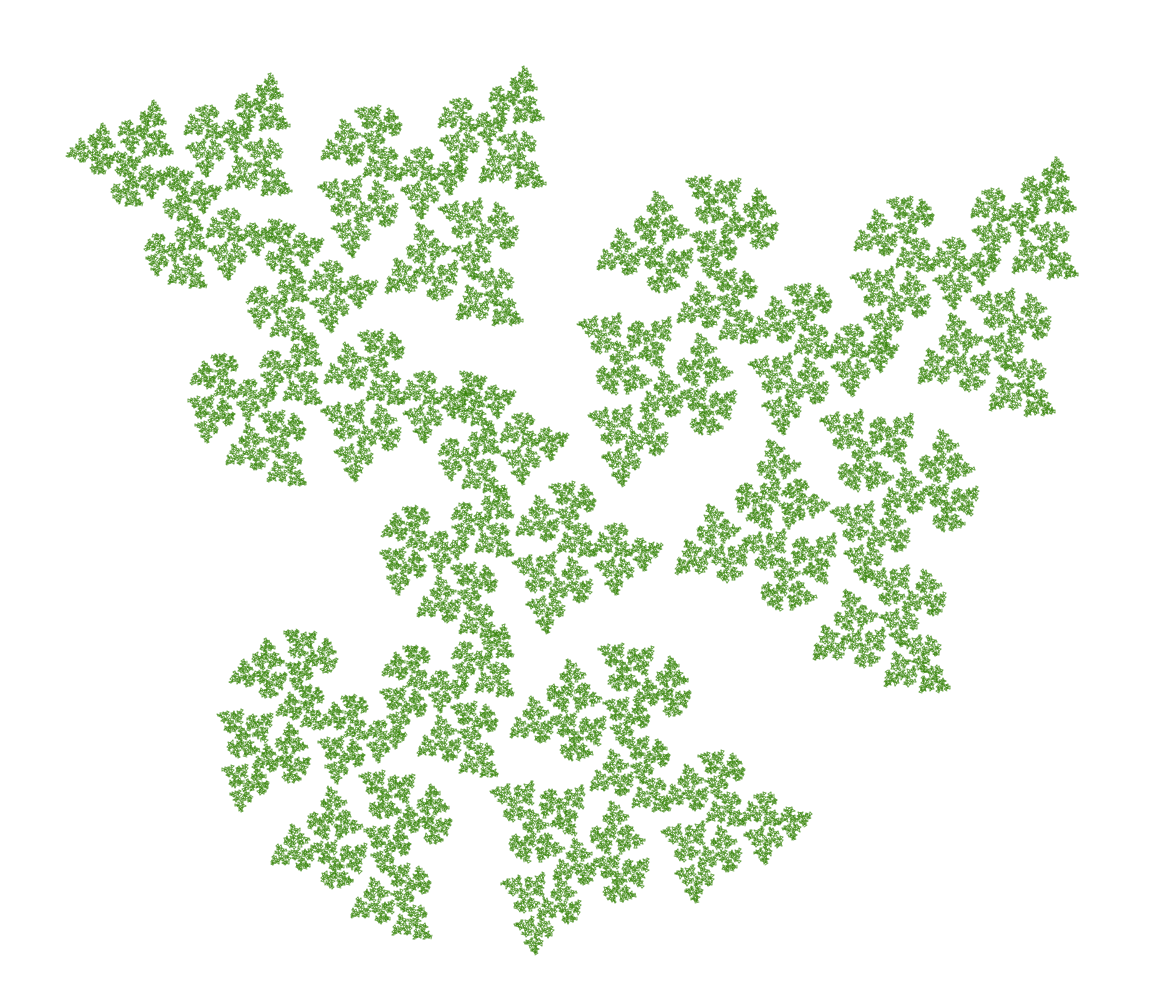
\includegraphics[width=0.6\textwidth]{img/Simple_Techniques/Unconnect/simple_un_triangle_01.png}}
        \end{figure}

        \FloatBarrier

        \begin{figure}[ht]
            \caption{\label{simple_un_quad_01} A unconnected transformation with a figure.}
            \centering
            \subcaptionbox{}[0.2\textwidth]
                {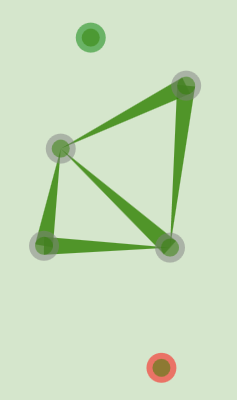
\includegraphics[width=0.2\textwidth]{img/Simple_Techniques/Unconnect/simple_un_setup_quad_01.png}}
            \subcaptionbox{}[0.7\textwidth]
                {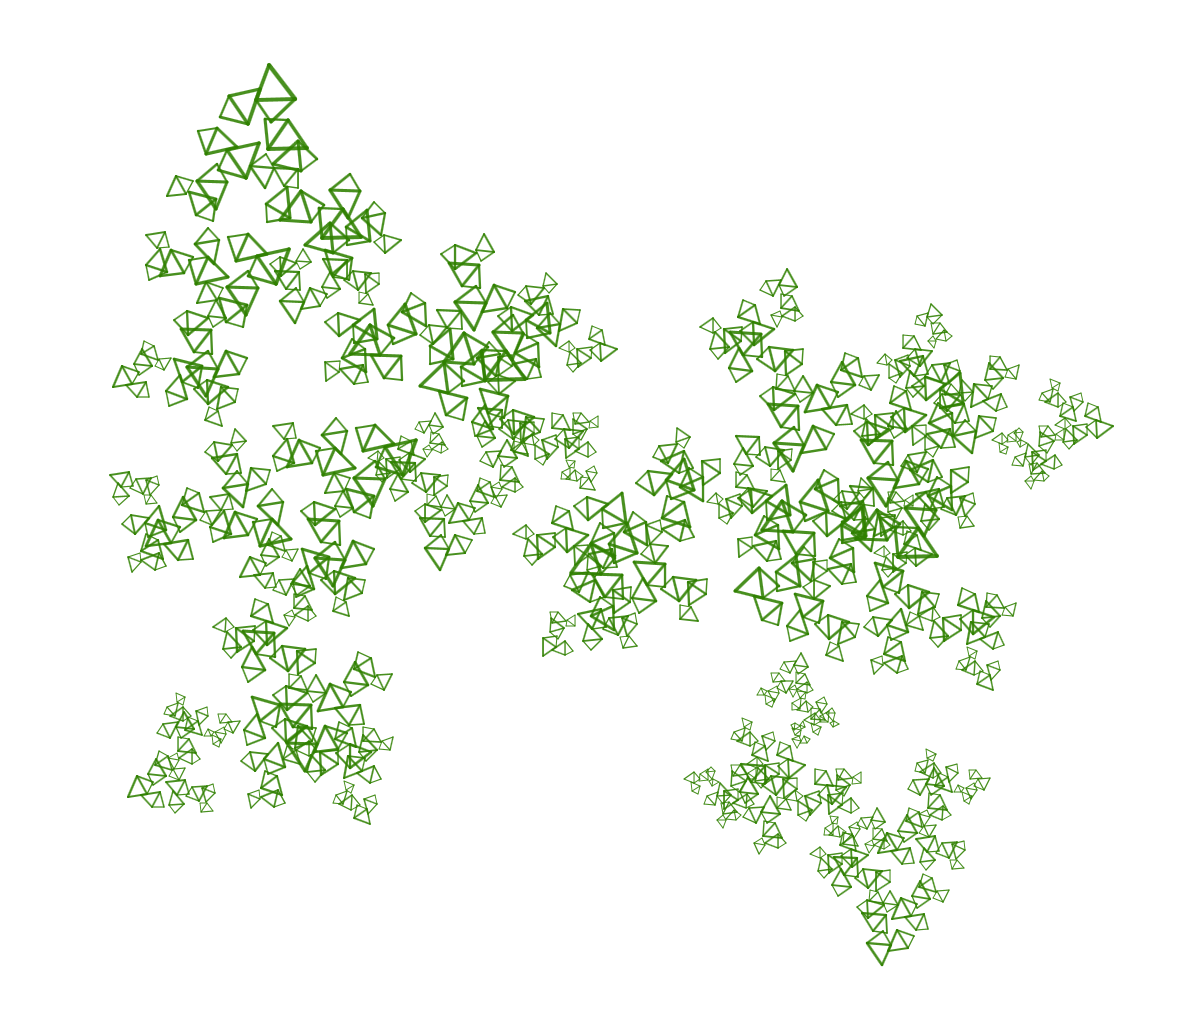
\includegraphics[width=0.6\textwidth]{img/Simple_Techniques/Unconnect/simple_un_quad_01.png}}
        \end{figure}

        \FloatBarrier

    \subsection{Singleton Pattern}

        Suppose we have the following setup (fig.~\ref{simple_singleton_01}).
        This is the dragon curve with a square inside.
        Looking at the fractal after some iterations (fig.~\ref{simple_singleton_02}) it is clear that this is not a very aesthetically pleasing fractal.
        It would be much better if only the squares from the last iterations were seen.

        \begin{figure}[ht]
            \caption{An example.}
            \centering
            \subcaptionbox{\label{simple_singleton_01} The setup.}[0.3\textwidth]
                {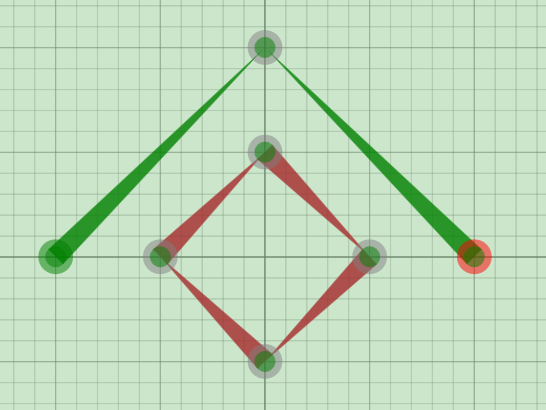
\includegraphics[width=0.3\textwidth]{img/Simple_Techniques/Singleton/simple_singleton_01.png}}
            \subcaptionbox{\label{simple_singleton_02} After some iterations}[0.65\textwidth]
                {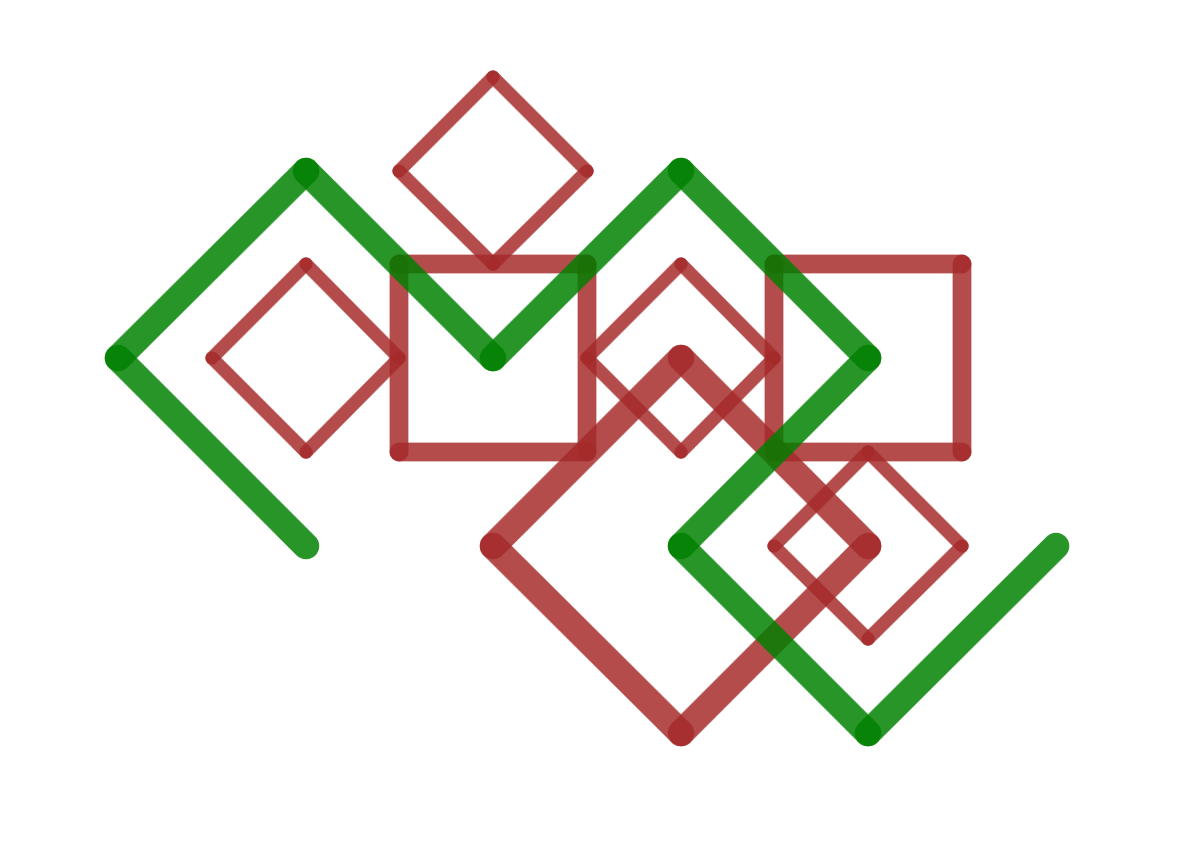
\includegraphics[width=0.6\textwidth]{img/Simple_Techniques/Singleton/simple_singleton_02.png}}
        \end{figure}

        The Singleton pattern solves this problem.
        First we need to create a new type of transformation (fig.~\ref{simple_single_03}).
        It may be strange that the transformation for a singleton pattern doesn't require any segments,
            but the value of this pattern will itself.

        \begin{figure}[ht]
            \caption{\label{simple_single_03} The singleton transformation.}
            \centering
            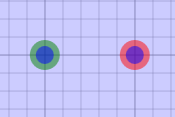
\includegraphics[width=0.3\textwidth]{img/Simple_Techniques/Singleton/simple_single_setup_02.png}
        \end{figure}

        Let's try to change the dragon curve example on more time, this time using the blue layer (fig.~\ref{simple_singleton_03}).
        In this case the final result looks like this (fig.~\ref{simple_singleton_04}).
        The logic behind this is quite clear, on every iteration a new pair of squares forms but the last one iterates into the singleton transformation and disappears.

        \begin{figure}[ht]
            \caption{Using the singleton pattern.}
            \centering
            \subcaptionbox{\label{simple_singleton_03} The setup.}[0.3\textwidth]
                {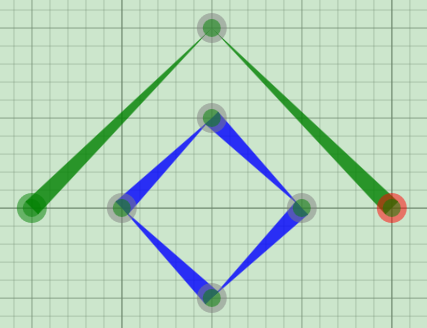
\includegraphics[width=0.3\textwidth]{img/Simple_Techniques/Singleton/simple_single_setup_03.png}}
            \subcaptionbox{\label{simple_singleton_04} After some iterations}[0.65\textwidth]
                {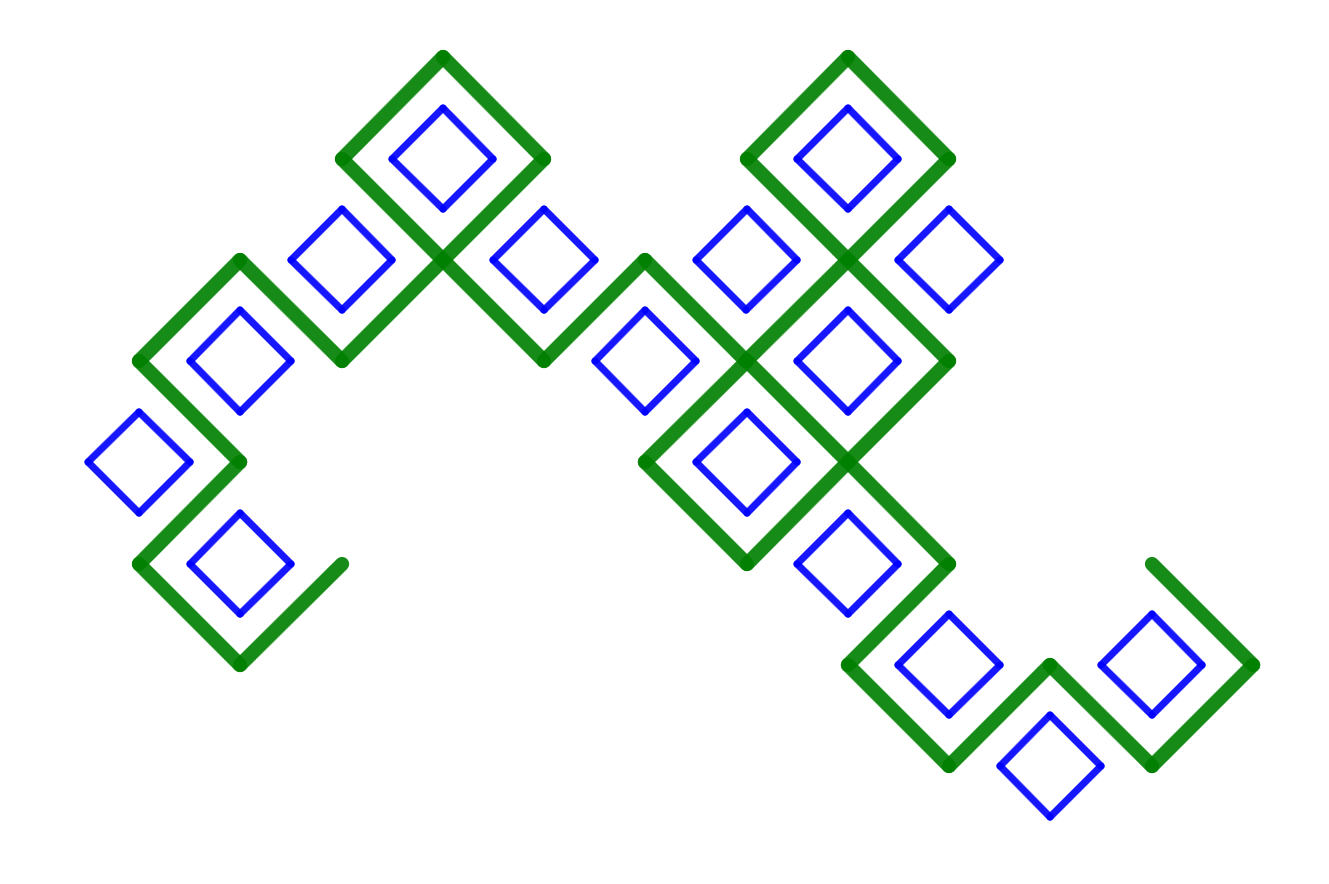
\includegraphics[width=0.6\textwidth]{img/Simple_Techniques/Singleton/simple_single_02.png}}
        \end{figure}

        \FloatBarrier

        Instead of just square we can use any type of figure (fig.\ref{simple_single_05}).

        \begin{figure}[ht]
            \caption{\label{simple_single_05} Some examples.}
            \centering
            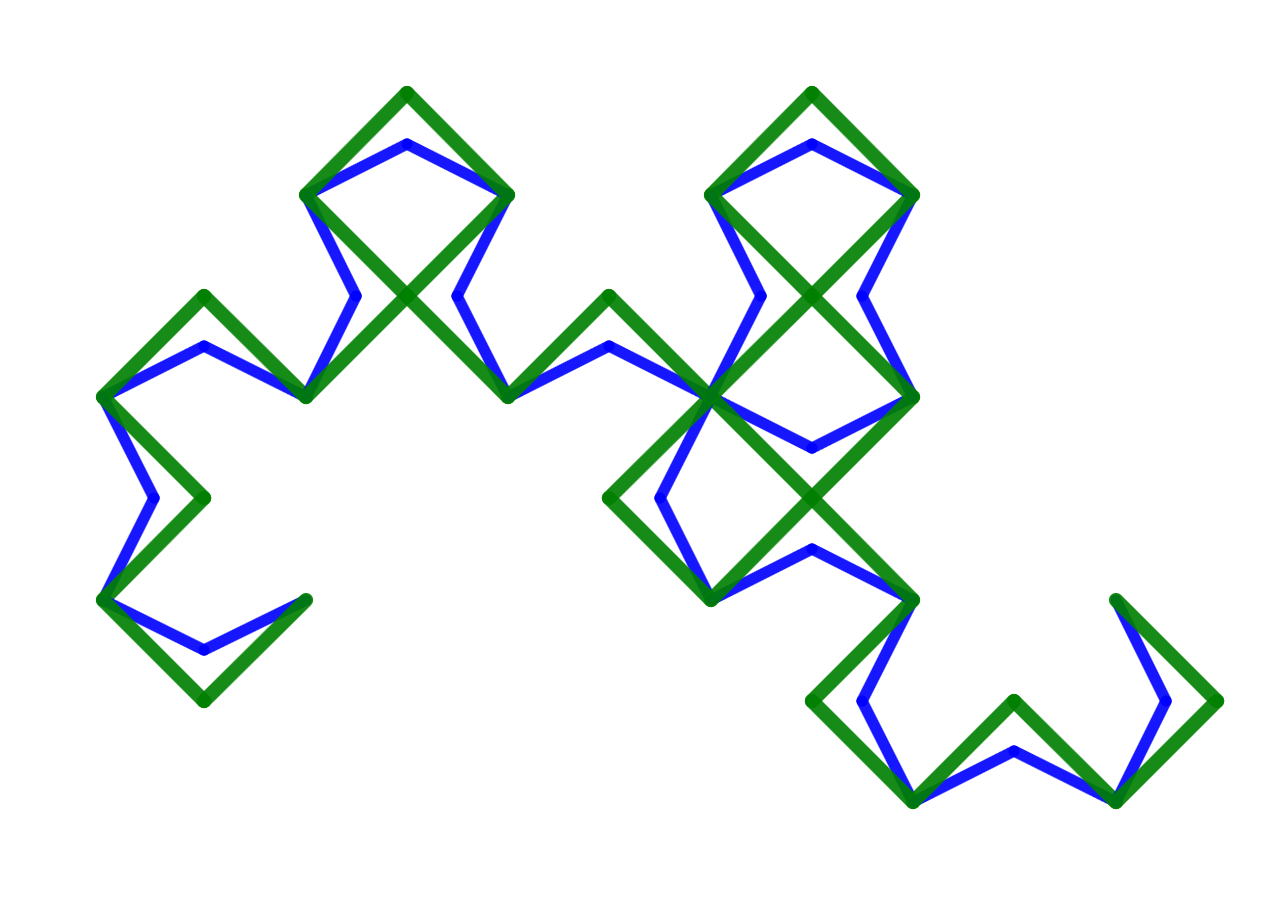
\includegraphics[width=0.4\textwidth]{img/Simple_Techniques/Singleton/simple_single_03.png}
            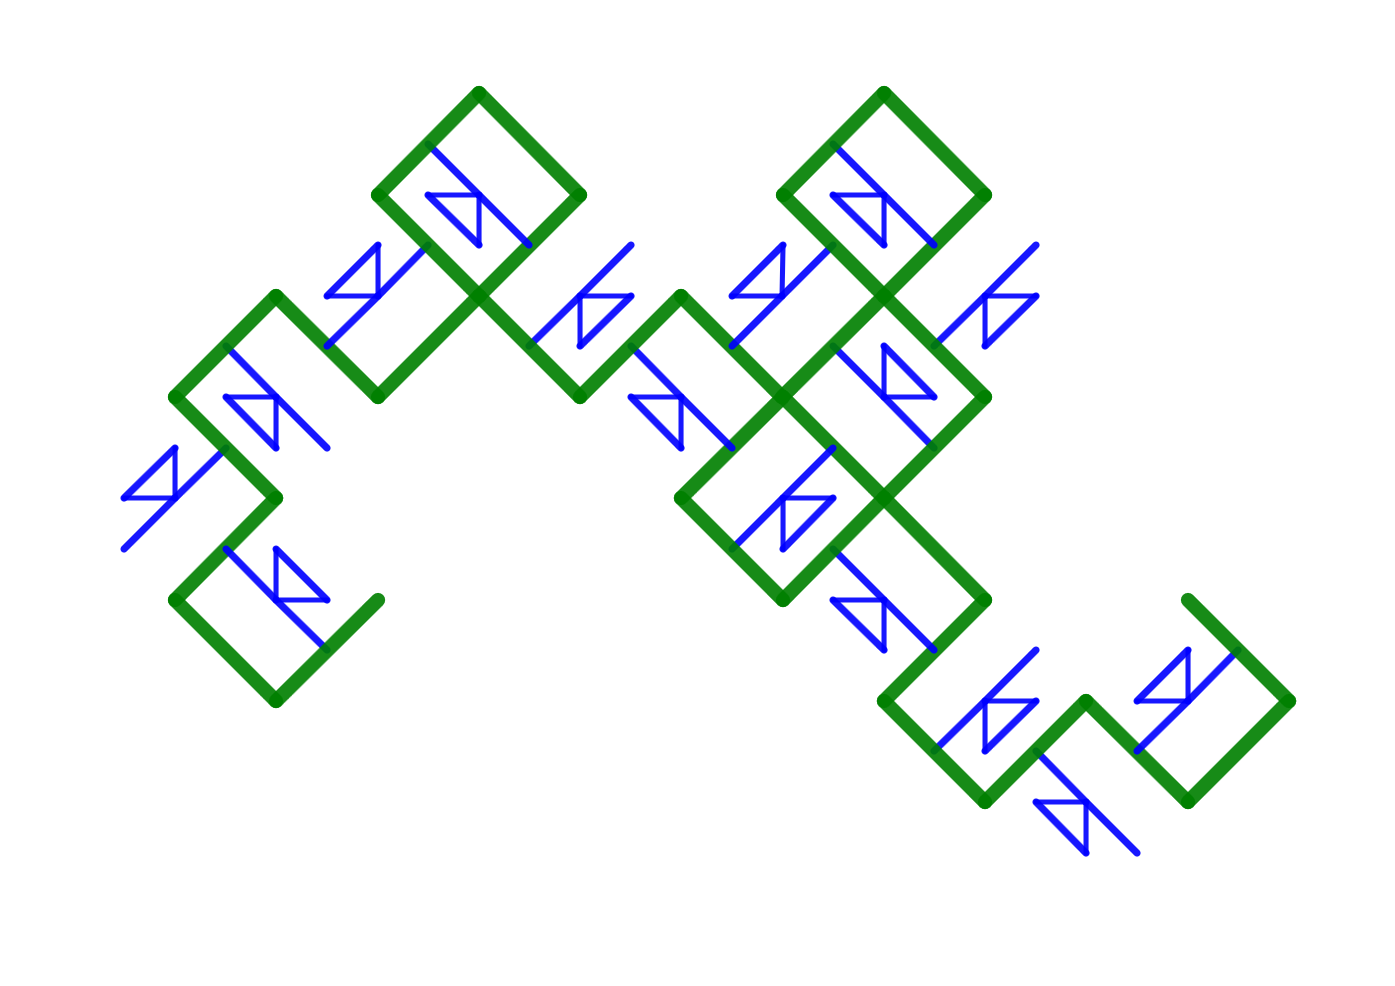
\includegraphics[width=0.4\textwidth]{img/Simple_Techniques/Singleton/simple_single_04.png}
        \end{figure}

        \FloatBarrier

        In the previous example only the dragon curve was used.
        This was due to the fact that it was easier to explain using it, nevertheless singleton pattern can be applied in a big variety of cases.
        

    \subsection{Decorator Pattern}

        The definition of the decorator pattern is more abstract than the definition of the previous patterns.
        The idea is to divide segments in two parts. 
        One that is responsible for the recursion mechanics and the other one responsible for the visual setup.

        Let's review the dragon curve example from the previous chapter but make some changes.
        We will use a singleton transformation and the setup will be the same (fig.~\ref{simple_singleton_03}).
        This time, however, I will use a interesting property of the software.
        Inside the color-choosing window there is a gray square with an X inside.
        Pressing that square will make the segments of this transformation completely transparent.
        In this way, the green segments will not be seen, only the blue squares.

        \begin{figure}[ht]
            \centering
            \subcaptionbox{}[0.3\textwidth]
                {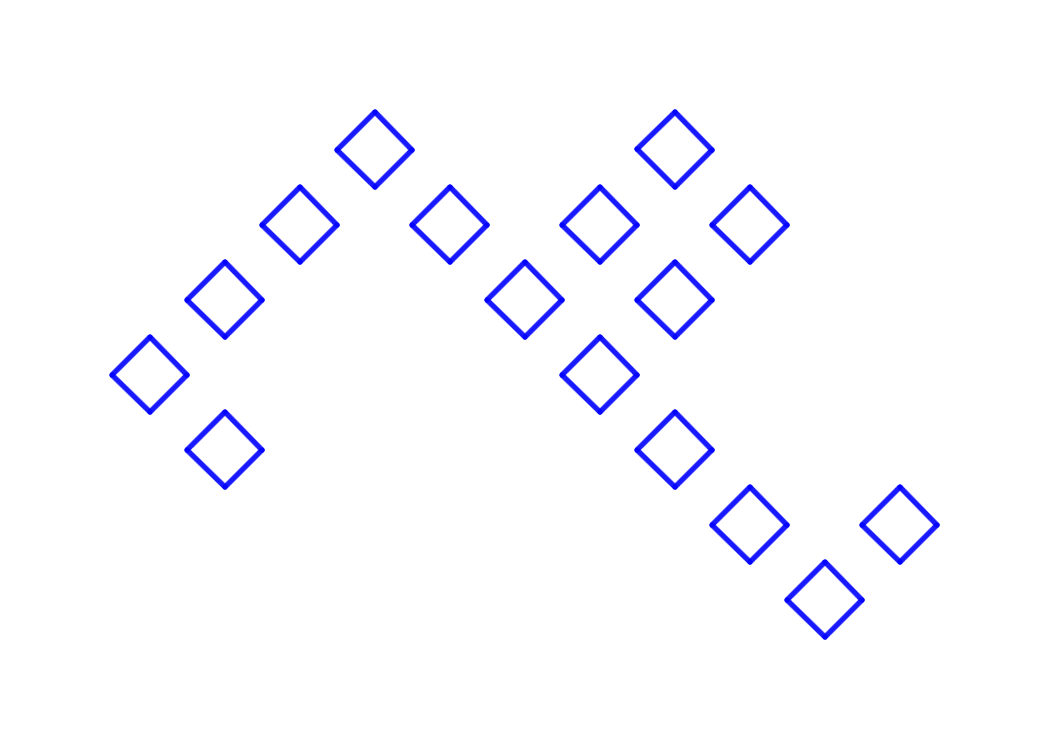
\includegraphics[width=0.3\textwidth]{img/Simple_Techniques/Decorator/simple_deco_01.png}}
            ~
            \subcaptionbox{}[0.6\textwidth]
                {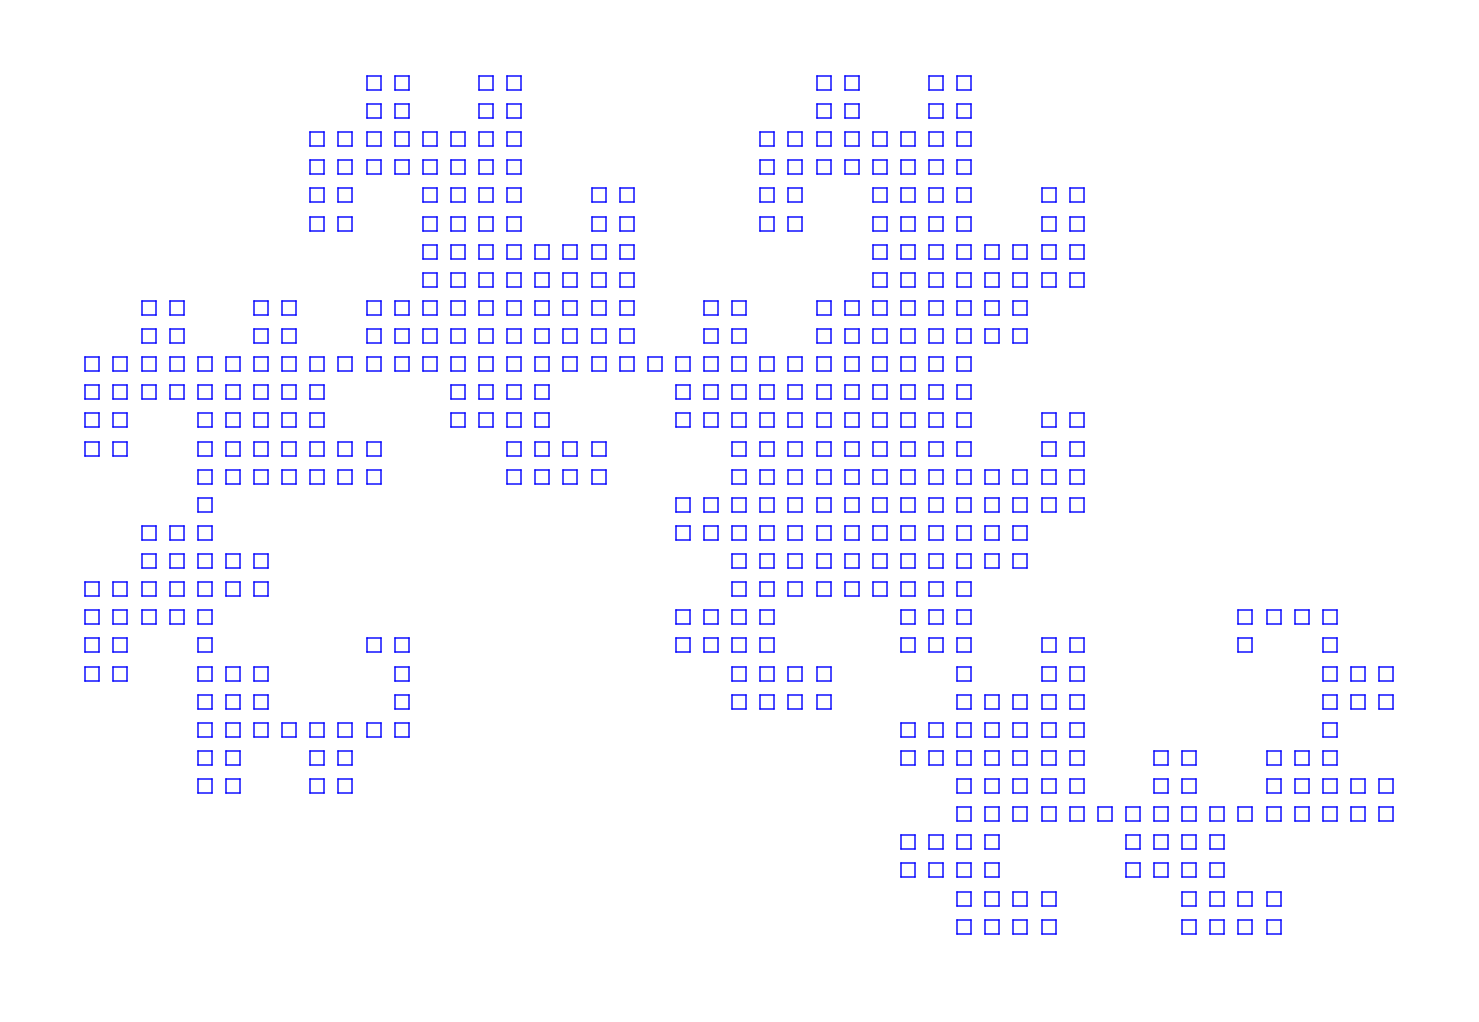
\includegraphics[width=0.6\textwidth]{img/Simple_Techniques/Decorator/simple_deco_02.png}}
        \end{figure}

    \subsection{Case Studies}
        
        \subsubsection{Two Rays}

            The title might be misleading since we are not actually dealing with mathematical rays.
            Figure~\ref{ray_01} shows the setup and the figure that it creates.

            \begin{figure}[H]
                \centering
                \caption{\label{ray_01} Two Rays}
                \subcaptionbox{The setup}[0.18\textwidth]
                    {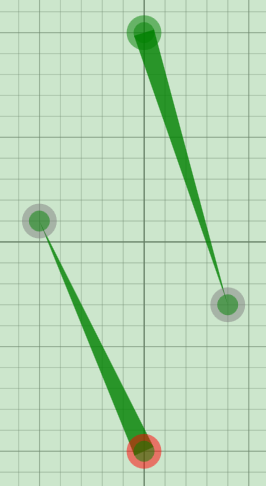
\includegraphics[width=0.18\textwidth]{img/Simple_Techniques/Cases/rays/ray_set_01.png}}
                ~
                \subcaptionbox{The fractal.}[0.78\textwidth]
                    {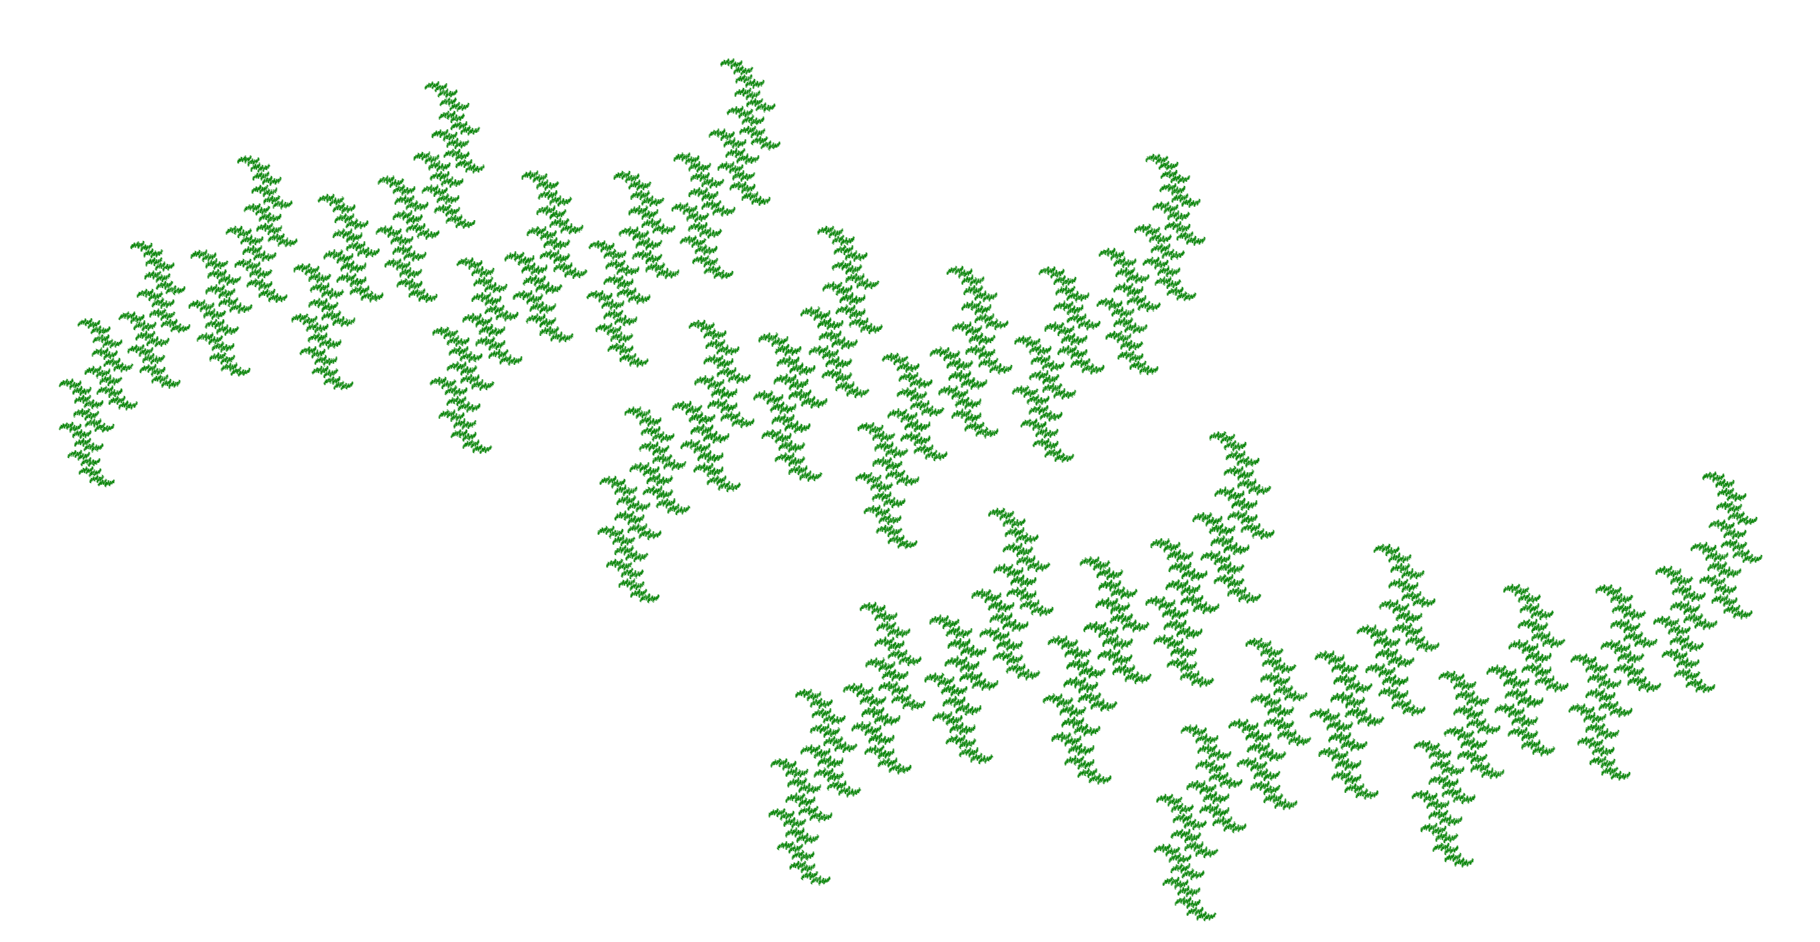
\includegraphics[width=0.78\textwidth]{img/Simple_Techniques/Cases/rays/ray_01.png}}
            \end{figure}

            It's probably clear why the name \quotes{Rays} was chosen.

            Since the segments are not connected to each other, the final fractal is unconnected.
            This doesn't mean that the segments cannot overlap, this is actually a very common feature of unconnected fractals.

            If we change the setup we can get an interesting fractal (fig.\ref{ray_02}).
            The fractal is similar to the Dragon Curve.
            Even though the segments are unconnected, this fractals shows a interesting type of connection.


            \begin{figure}[H]
                \centering
                \caption{\label{ray_02} The Ray Dragon.}
                \subcaptionbox{The setup}[0.3\textwidth]
                    {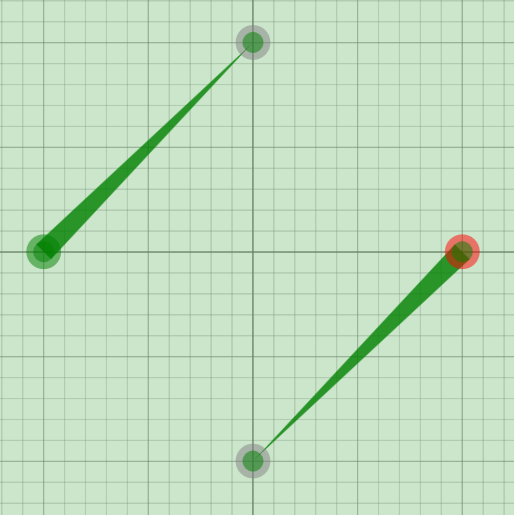
\includegraphics[width=0.3\textwidth]{img/Simple_Techniques/Cases/rays/ray_set_02.png}}
                ~
                \subcaptionbox{The fractal.}[0.65\textwidth]
                    {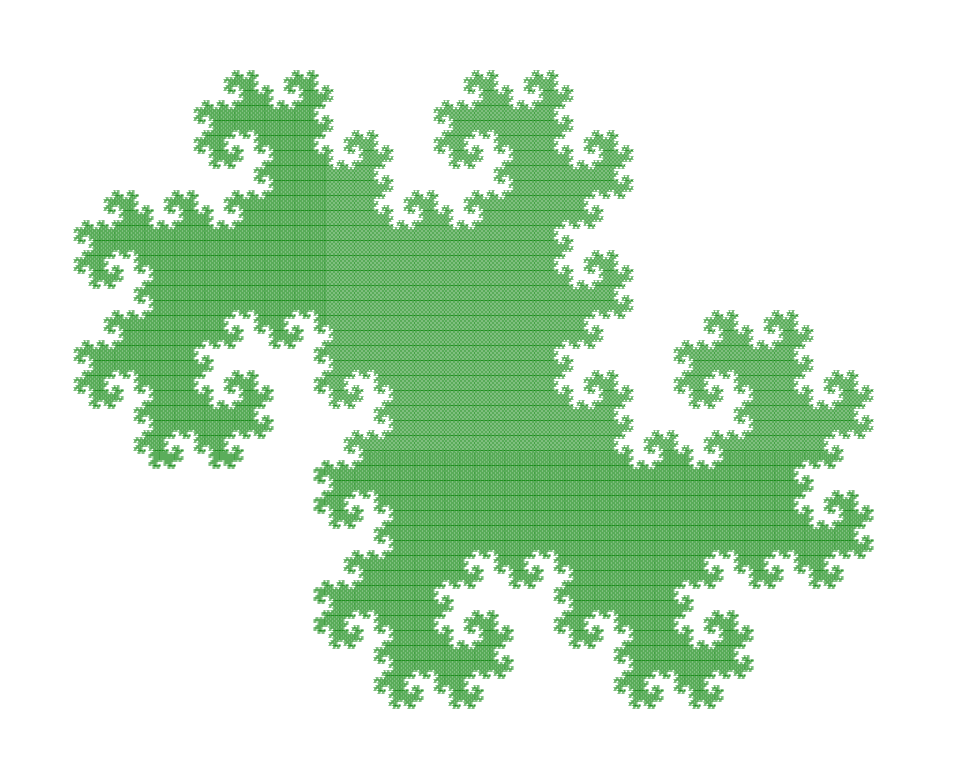
\includegraphics[width=0.65\textwidth]{img/Simple_Techniques/Cases/rays/ray_02.png}}

                \subcaptionbox{First iterations.}[1\textwidth]
                    {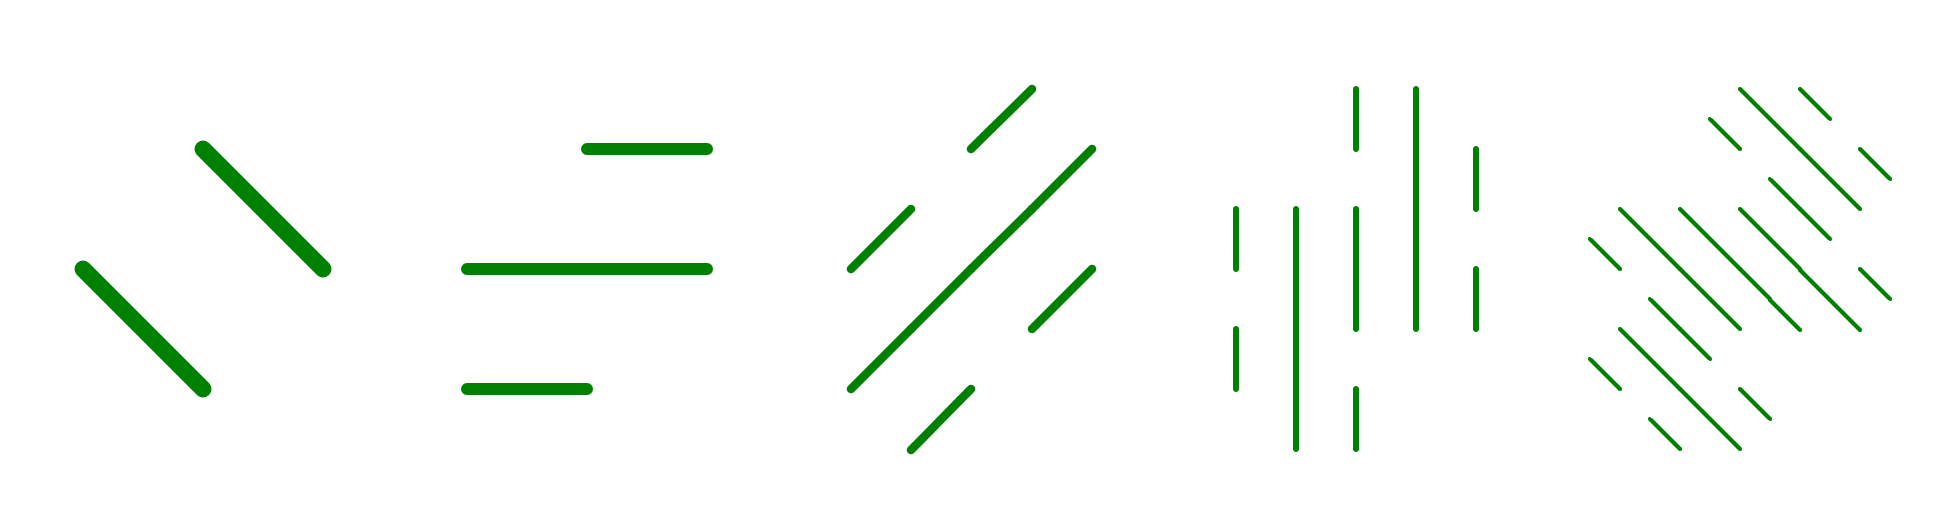
\includegraphics[width=1\textwidth]{img/Simple_Techniques/Cases/rays/ray_03.png}}
            \end{figure}

            Moving the segments around we can get other types of strange fractals.
            We can try to invert the arrows, that is, change their direction.
            There are 4 combination in total, below are all the combination applied to the same set of points.

            \begin{figure}[H]
                \centering
                \caption{\label{ray_04} Combination 1.}
                \subcaptionbox{The setup}[0.2\textwidth]
                    {\includegraphics[width=0.2\textwidth]{img/Simple_Techniques/Cases/rays/ray_set_04.png}}
                ~
                \subcaptionbox{The fractal.}[0.78\textwidth]
                    {\includegraphics[width=0.78\textwidth]{img/Simple_Techniques/Cases/rays/ray_04.png}}
            \end{figure}

            \begin{figure}[H]
                \centering
                \caption{\label{ray_06} Combination 2.}
                \subcaptionbox{The setup}[0.2\textwidth]
                    {\includegraphics[width=0.2\textwidth]{img/Simple_Techniques/Cases/rays/ray_set_06.png}}
                ~
                \subcaptionbox{The fractal.}[0.78\textwidth]
                    {\includegraphics[width=0.78\textwidth]{img/Simple_Techniques/Cases/rays/ray_06.png}}
            \end{figure}

            \begin{figure}[H]
                \centering
                \caption{\label{ray_05} Combination 3.}
                \subcaptionbox{The setup}[0.2\textwidth]
                    {\includegraphics[width=0.2\textwidth]{img/Simple_Techniques/Cases/rays/ray_set_05.png}}
                ~
                \subcaptionbox{The fractal.}[0.78\textwidth]
                    {\includegraphics[width=0.78\textwidth]{img/Simple_Techniques/Cases/rays/ray_05.png}}
            \end{figure}

            

            \begin{figure}[H]
                \centering
                \caption{\label{ray_07} Combination 4.}
                \subcaptionbox{The setup}[0.2\textwidth]
                    {\includegraphics[width=0.2\textwidth]{img/Simple_Techniques/Cases/rays/ray_set_07.png}}
                ~
                \subcaptionbox{The fractal.}[0.78\textwidth]
                    {\includegraphics[width=0.78\textwidth]{img/Simple_Techniques/Cases/rays/ray_07.png}}
            \end{figure}


            As we can observe the long segment changes the general aspect of the fractal whilst the smaller ones changes the details of the fractal.

            As a final note, the small segment can be substituted with anything else, for example a tree.

            \begin{figure}[H]
                \centering
                \caption{\label{ray_08} Tree in spiral.}
                \includegraphics[width=0.6\TW]{img/Simple_Techniques/Cases/rays/ray_08.png}
            \end{figure}